\documentclass[12pt]{article}

% Автор: Илья Дудников
% Автор стиля: Сергей Копелиович

\usepackage{cmap}
\usepackage[T2A]{fontenc}
\usepackage[utf8]{inputenc}
\usepackage[russian]{babel}
\usepackage{graphicx}
\usepackage{amsthm,amsmath,amssymb}
\usepackage{listings}
\usepackage{color}
\usepackage{array}
\usepackage{epigraph}
\usepackage{multicol}
\usepackage{cancel}
\usepackage{float}
\usepackage{wrapfig}
\usepackage{caption}
\usepackage{subcaption}

\usepackage[usenames,dvipsnames]{xcolor}
\usepackage[russian,colorlinks=true,urlcolor=red,linkcolor=blue]{hyperref}
\usepackage{enumerate}
\usepackage{datetime}
\usepackage{fancyhdr}
\usepackage{lastpage}
\usepackage{verbatim}
\usepackage{tikz}
\usepackage{MnSymbol}
\usetikzlibrary{arrows,decorations.markings,decorations.pathmorphing}
\usepackage{pgfplots}
\usepackage{ifthen}
\usepackage{mathtools}
\usepackage{mathrsfs}

%\usepackage{tabls}
%\usepackage{tabularx}
%\usepackage{xifthen}
%\listfiles

\def\NAME{Лекции}
\def\SEASON{Конспект лекций по дискретной математике, ПИ, 2 семестр}

\sloppy
\voffset=-20mm
\textheight=235mm
\hoffset=-22mm
\textwidth=180mm
\headsep=12pt
\footskip=20pt

\parskip=0em
\parindent=0em

\setlength\epigraphwidth{.8\textwidth}

\newlength{\tmplen}
\newlength{\tmpwidth}
\newcounter{listcounter}

% Список с маленькими отступами
\newenvironment{MyList}[1][4pt]{
  \begin{enumerate}[1.]
  \setlength{\parskip}{0pt}
  \setlength{\itemsep}{#1}
}{       
  \end{enumerate}
}
% Вложенный список с маленькими отступами
\newenvironment{InnerMyList}[1][0pt]{
  \vspace*{-0.5em}
  \begin{enumerate}[(a)]
  \setlength{\parskip}{-0pt}
  \setlength{\itemsep}{#1}
}{       
  \end{enumerate}
  \vspace*{-0.5em}
}
% Список с маленькими отступами
\newenvironment{MyItemize}[1][4pt]{
  \begin{itemize}
  \setlength{\parskip}{0pt}
  \setlength{\itemsep}{#1}
}{       
  \end{itemize}
}

% Основные математические символы
\def\TODO{{\color{red}\bf TODO}}
\def\C{\mathbb{C}}       %
\def\Q{\mathbb{Q}}       %
\def\N{\mathbb{N}}       %
\def\R{\mathbb{R}}       %
\def\F2{\mathbb{F}_2}    %
\def\Z{\mathbb{Z}}       %
\def\INF{\t{+}\infty}    % +inf
\def\EPS{\varepsilon}    %
\def\EMPTY{\varnothing}  %
\def\PHI{\varphi}        %
\def\SO{\Rightarrow}     % =>
\def\EQ{\Leftrightarrow} % <=>
\def\t{\texttt}          % mono font
\def\c#1{{\rm\sc{#1}}}   % font for classes NP, SAT, etc
\def\O{\mathcal{O}}      %
\def\NO{\t{\#}}          % #
\def\XOR{\text{ {\raisebox{-2pt}{\ensuremath{\Hat{}}}} }}
\renewcommand{\le}{\leqslant}
\renewcommand{\ge}{\geqslant}
\newcommand{\q}[1]{\langle #1 \rangle}               % <x>
\newcommand\URL[1]{{\footnotesize{\url{#1}}}}        %
% \newcommand{\sfrac}[2]{{\scriptscriptstyle\frac{#1}{#2}}}  % Очень маленькая дробь
% \newcommand{\mfrac}[2]{{\scriptstyle\frac{#1}{#2}}}    % Небольшая дробь
\newcommand{\sfrac}[2]{{\scriptstyle\frac{#1}{#2}}}  % Очень маленькая дробь
\newcommand{\mfrac}[2]{{\textstyle\frac{#1}{#2}}}    % Небольшая дробь

\newcommand{\fix}[1]{{\color{fixcolor}{#1}}} % \underline
\def\bonus{\t{\red{(*)}}}
\def\ifbonus#1{\ifthenelse{\equal{#1}{}}{}{\bonus}}
\def\smallsquare{$\scalebox{0.5}{$\square$}$}

\newlength{\myItemLength}
\setlength{\myItemLength}{0.3em}
\def\ItemSymbol{\smallsquare}
\def\Item{\vspace*{\myItemLength}\ItemSymbol \ \ }

\newcommand{\LET}{%
  % [line width=0.6pt]
  \begin{tikzpicture}%
  \draw(0.8ex,0) -- (0.8ex,1.6ex);%
  \draw(0,1.6ex) -- (0.8ex,1.6ex);%
  \end{tikzpicture}%
  \hspace*{0.1em}%
}

% Отступы
\def\makeparindent{\hspace*{\parindent}\unskip}
\def\up{\vspace*{-0.5em}}%{\vspace*{-\baselineskip}}
\def\down{\vspace*{0.5em}}
\def\LINE{\vspace*{-1em}\noindent \underline{\hbox to 1\textwidth{{ } \hfil{ } \hfil{ } }}}
\def\BOX#1{\mbox{\fbox{\bf{#1}}}}
\def\Pagebreak{\pagebreak\vspace*{-1.5em}}

% Мелкий заголовок
\newcommand{\THEE}[1]{
  \vspace*{0.5em}
  \noindent{\bf \underline{#1}}%\hspace{0.5em}
  \vspace*{0.2em}
}
% Другой тип мелкого заголовка
\newcommand{\THE}[1]{
  \vspace*{0.5em} $\bullet$
  \noindent{\bf #1}%\hspace{0.5em}
  \vspace*{0.2em}
}

\newenvironment{MyTabbing}{
  \t\bgroup
  \vspace*{-\baselineskip}
  \begin{tabbing}
    aaaa\=aaaa\=aaaa\=aaaa\=aaaa\=aaaa\kill
}{
  \end{tabbing}
  \t\egroup
}

% Код с правильными отступами
\lstnewenvironment{code}{
  \lstset{}
%  \vspace*{-0.2em}
}%
{
%  \vspace*{-0.2em}
}
\lstnewenvironment{codep}{
  \lstset{language=python}
}%
{
}

% Формулы с правильными отступами
\newenvironment{smallformula}{
 
  \vspace*{-0.8em}
}{
  \vspace*{-1.2em}
  
}
\newenvironment{formula}{
 
  \vspace*{-0.4em}
}{
  \vspace*{-0.6em}
  
}

% Большая квадратная скобка
\makeatletter
\newenvironment{sqcases}{%
  \matrix@check\sqcases\env@sqcases
}{%
  \endarray\right.%
}
\def\env@sqcases{%
  \let\@ifnextchar\new@ifnextchar
  \left\lbrack
  \def\arraystretch{1.2}%
  \array{@{}l@{\quad}l@{}}%
}
\makeatother

% theorems
\makeatother
\usepackage{thmtools}
\usepackage[framemethod=TikZ]{mdframed}
\mdfsetup{skipabove=1em,skipbelow=0em}


\theoremstyle{definition}

\declaretheoremstyle[
    headfont=\bfseries\sffamily\color{ForestGreen!70!black}, bodyfont=\normalfont,
    mdframed={
        linewidth=2pt,
        rightline=false, topline=false, bottomline=false,
        linecolor=ForestGreen, backgroundcolor=ForestGreen!5,
    }
]{thmgreenbox}

\declaretheoremstyle[
    headfont=\bfseries\sffamily\color{NavyBlue!70!black}, bodyfont=\normalfont,
    mdframed={
        linewidth=2pt,
        rightline=false, topline=false, bottomline=false,
        linecolor=NavyBlue, backgroundcolor=NavyBlue!5,
    }
]{thmbluebox}

\declaretheoremstyle[
    headfont=\bfseries\sffamily\color{NavyBlue!70!black}, bodyfont=\normalfont,
    mdframed={
        linewidth=2pt,
        rightline=false, topline=false, bottomline=false,
        linecolor=NavyBlue
    }
]{thmblueline}

\declaretheoremstyle[
    headfont=\bfseries\sffamily\color{RawSienna!70!black}, bodyfont=\normalfont,
    mdframed={
        linewidth=2pt,
        rightline=false, topline=false, bottomline=false,
        linecolor=RawSienna, backgroundcolor=RawSienna!5,
    }
]{thmredbox}

\declaretheoremstyle[
    headfont=\bfseries\sffamily\color{RawSienna!70!black}, bodyfont=\normalfont,
    numbered=no,
    mdframed={
        linewidth=2pt,
        rightline=false, topline=false, bottomline=false,
        linecolor=RawSienna, backgroundcolor=RawSienna!1,
    },
    qed=\qedsymbol
]{thmproofbox}

\declaretheoremstyle[
    headfont=\bfseries\sffamily\color{NavyBlue!70!black}, bodyfont=\normalfont,
    numbered=no,
    mdframed={
        linewidth=2pt,
        rightline=false, topline=false, bottomline=false,
        linecolor=NavyBlue, backgroundcolor=NavyBlue!1,
    },
]{thmexplanationbox}

\declaretheorem[style=thmgreenbox, name=Определение]{Def}
\declaretheorem[style=thmbluebox, numbered=no, name=Пример]{Example}
\declaretheorem[style=thmredbox, name=Утверждение]{Prop}
\declaretheorem[style=thmredbox, name=Теорема]{Thm}
\declaretheorem[style=thmredbox, name=Алгоритм]{Algo}
\declaretheorem[style=thmredbox, name=Свойство]{Property}
\declaretheorem[style=thmredbox, name=Лемма]{Lm}
\declaretheorem[style=thmredbox, numbered=no, name=Следствие]{Cons}

\declaretheorem[style=thmproofbox, name=Доказательство]{replacementproof}
\renewenvironment{proof}[1][\proofname]{\vspace{-10pt}\begin{replacementproof}}{\end{replacementproof}}


\declaretheorem[style=thmexplanationbox, name=Доказательство]{tmpexplanation}
\newenvironment{explanation}[1][]{\vspace{-10pt}\begin{tmpexplanation}}{\end{tmpexplanation}}

\declaretheorem[style=thmblueline, numbered=no, name=Замечание]{Rem}
\declaretheorem[style=thmblueline, numbered=no, name=Note]{note}

\newtheorem*{notation}{Обозначение}
\newtheorem*{Ex}{Упражнение}

% Определяем основные секции: \begin{Lm}, \begin{Thm}, \begin{Def}, \begin{Rem}
% \renewcommand{\qedsymbol}{$\blacksquare$}
% \theoremstyle{definition} % жирный заголовок, плоский текст
% \newtheorem{Thm}{\underline{Теорема}}[subsection] % нумерация будет "<номер subsection>.<номер теоремы>"
% \newtheorem{Lm}[Thm]{\underline{Lm}} % Нумерация такая же, как и у теорем
% \newtheorem{Ex}[Thm]{Упражнение} % Нумерация такая же, как и у теорем
% \newtheorem{Example}[Thm]{Пример} % Нумерация такая же, как и у теорем
% \newtheorem{Code}[Thm]{Код} % Нумерация такая же, как и у теорем
% \theoremstyle{plain} % жирный заголовок, курсивный текст
% \newtheorem{Def}[Thm]{Def} % Нумерация такая же, как и у теорем
% \theoremstyle{remark} % курсивный заголовок, плоский текст
% \newtheorem{Cons}[Thm]{Следствие} % Нумерация такая же, как и у теорем
% \newtheorem{Conj}[Thm]{Гипотеза} % Нумерация такая же, как и у теорем
% \newtheorem{Prop}[Thm]{Утверждение} % Нумерация такая же, как и у теорем
% \newtheorem{Rem}[Thm]{Замечание} % Нумерация такая же, как и у теорем
% \newtheorem{Remark}[Thm]{Замечание} % Нумерация такая же, как и у теорем
% \newtheorem{Algo}[Thm]{Алгоритм} % Нумерация такая же, как и у теорем

% Определяем ЗАГОЛОВКИ
\def\SectionName{unknown}
\def\AuthorName{unknown}

\newlength{\sectionvskip}
\setlength{\sectionvskip}{0.5em}
\newcommand{\Section}[4][]{
  % Заголовок
  \pagebreak
%  \ifthenelse{\isempty{#1}}{
    \refstepcounter{section}
%  }{}
  \vspace{0.5em}
%  \ifthenelse{\isempty{#1}}{
%    \addtocontents{toc}{\protect\addvspace{-5pt}}%
    \addcontentsline{toc}{section}{\arabic{section}. #2}
%  }{}
  \begin{center}
    {\Large \bf Раздел \NO{\arabic{section}}: #2} \\ 
    \vspace{\sectionvskip}
    \ifthenelse{\equal{#3}{}}{}{{\large #3}\\}
  \end{center}

  \LINE

  % Запомнили название и автора главы
  \gdef\SectionName{#2}
  \gdef\AuthorName{#4}

  % Заголовок страницы
  \lhead{\SEASON}
  \chead{}
  \rhead{\SectionName}
  \renewcommand{\headrulewidth}{0.4pt}

  \lfoot{Глава \NO{\arabic{section}}.}
  \cfoot{\thepage\t{/}\pageref*{LastPage}}
  \rfoot{Автор: \AuthorName}
  \renewcommand{\footrulewidth}{0.4pt}
}

\newcommand{\Subsection}[2][]{
  \refstepcounter{subsection}
  \vspace*{1em}
  \ifthenelse{\equal{#1}{}}
    {\addcontentsline{toc}{subsection}{\arabic{section}.\arabic{subsection}. #2}}
    {\addcontentsline{toc}{subsection}{\arabic{section}.\arabic{subsection}. \bonus\,#2}}
  {\color{blue}\bf\large \arabic{section}.\arabic{subsection}. \ifbonus{#1}\,{#2}} 
  \vspace*{0.5em}
  \makeparindent
}
\newcommand{\Subsubsection}[2][]{
  \refstepcounter{subsubsection}
  \vspace*{1em}
  \ifthenelse{\equal{#1}{}}
    {\addcontentsline{toc}{subsubsection}{\arabic{section}.\arabic{subsection}.\arabic{subsubsection}. #2}}
    {\addcontentsline{toc}{subsubsection}{\arabic{section}.\arabic{subsection}.\arabic{subsubsection}. \bonus\,#2}}
  {\color{blue}\bf\large \arabic{section}.\arabic{subsection}.\arabic{subsubsection}. \ifbonus{#1}\,#2}
  \vspace*{0.5em}
  \makeparindent
}

\makeatletter
\newcommand*{\encircled}[1]{\relax\ifmmode\mathpalette\@encircled@math{#1}\else\@encircled{#1}\fi}
\newcommand*{\@encircled@math}[2]{\@encircled{$\m@th#1#2$}}
\newcommand*{\@encircled}[1]{%
  \tikz[baseline,anchor=base]{\node[draw,circle,outer sep=0pt,inner sep=.2ex] {#1};}}
\makeatother

\newcommand{\Header}{
  \pagestyle{empty}
  \renewcommand{\dateseparator}{--}
  \begin{center}
    {\Large\bf 
     Дискретная математика \\ 2 семестр ПИ,\\
    \vspace{0.3em}
    \NAME}\\
    \vspace{0.7em}
    {Собрано {\today} в {\currenttime}}
  \end{center}

  \LINE
  \vspace{0em}

  \renewcommand{\baselinestretch}{0.98}\normalsize
  \tableofcontents
  \renewcommand{\baselinestretch}{1.0}\normalsize
  \pagebreak
}

\newcommand{\BeginConspect}{
  \pagestyle{fancy}
  \setcounter{page}{1}
}

\definecolor{mygray}{rgb}{0.7,0.7,0.7}
\definecolor{ltgray}{rgb}{0.9,0.9,0.9}
\definecolor{fixcolor}{rgb}{0.7,0,0}
\definecolor{red2}{rgb}{0.7,0,0}
\definecolor{dkred}{rgb}{0.4,0,0}
\definecolor{dkblue}{rgb}{0,0,0.6}
\definecolor{dkgreen}{rgb}{0,0.6,0}
\definecolor{brown}{rgb}{0.5,0.5,0}

\newcommand{\green}[1]{{\color{green}{#1}}}
\newcommand{\black}[1]{{\color{black}{#1}}}
\newcommand{\red}[1]{{\color{red}{#1}}}
\newcommand{\dkred}[1]{{\color{dkred}{#1}}}
\newcommand{\blue}[1]{{\color{blue}{#1}}}
\newcommand{\dkgreen}[1]{{\color{dkgreen}{#1}}}

\newcommand{\Mod}[1]{\ (\mathrm{mod}\ #1)}

\DeclareMathOperator{\Real}{Re}
\DeclareMathOperator{\Imag}{Im}
\DeclareMathOperator{\lcm}{lcm}
\DeclareMathOperator{\sign}{sign}
\DeclareMathOperator{\Si}{Si}
\DeclareMathOperator{\const}{const}
\DeclareMathOperator{\Arg}{Arg}

\begin{document}
	\Header

	\BeginConspect

	\Section{Аналитическая геометрия}{}{Илья Дудников}

	\Subsection{Системы координат}
	
	\Subsubsection{Аффинные системы координат}

	\begin{Def}
		Аффинной системой координат на прямой называется взаимно-однозначное соответствие $l \longleftrightarrow \R$. \\
		
		Она определяется выбором точки $O$  и выбором вектора $\overline{e}$. АСК = $\{O, \{\overline{e}\}\}$.
	\end{Def}

	\begin{figure*}[h]
		\centering
		\def\svgwidth{0.3\columnwidth}
		\input{img/as_line.pdf_tex}
	\end{figure*}


	\begin{Def}
		АСК на плоскости называется биекция $\pi \longleftrightarrow \R^2$. 

		Она определяется выбором точки $O$ и векторов $\overline{e}_1, \overline{e}_2 \neq \overline{e}_1, \overline{e}_1 \not\parallel \overline{e}_2$. 
		АСК = $\{O, \{\overline{e}_1, \overline{e}_2\}\}$.
	\end{Def}

	\begin{figure*}[h]
		\centering
		\def\svgwidth{0.3\columnwidth}
		\input{img/as_plane.pdf_tex}
	\end{figure*}

	\begin{Def}
		Если $|\overline{e}_1| = |\overline{e}_2| = 1, \overline{e}_1 \perp \overline{e}_2$, то АСК называется декартовой системой координат. 
	\end{Def}

	\begin{Def}
		АСК в пространстве называется биекция $M \longleftrightarrow \R^3$ .
		Она определяется выбором точки $O$ и векторов $\overline{e}_1, \overline{e}_2, \overline{e}_3 \neq \overline{0}$ -- не компланарны. АСК = $\{O, \{\overline{e}_1, \overline{e}_2, \overline{e}_3\}\}$.
	\end{Def}

	\begin{Def}
		Упорядоченная тройка векторов $(\overline{u}, \overline{v}, \overline{w})$ называется \textbf{правой} , 
		если из конца вектора $\overline{w}$ поворот то $\overline{u}$ к $\overline{v}$ по наименьшему углу выглядит происходящим против часовой стрелки,
		и \textbf{левой} -- в противном случае. 
	\end{Def}

	\Pagebreak
	\Subsubsection{Криволинейные системы координаты}

	\begin{Def}
		Выберем точку $O$ и построим из неё луч $p$, который назовем \textit{полярной осью}. Возьмем теперь произвольную точку $M$ на плоскости и измерим две величины:
		расстояние от $M$ до $O$ и угол между вектором $\overline{OM}$ и полярной осью. Обозначим расстояние за $r$, а угол за $\PHI$.
		Тогда, чтобы избежать неоднозначности, будем считать, что $r > 0, \PHI \in [0, 2\pi)$, и если $r = 0$, то $\PHI = 0$.    
		Такая система координат называется \textbf{полярной}.		

	\end{Def}

	\begin{figure*}[h]
		\centering
		\def\svgwidth{0.3\columnwidth}
		\input{img/polar_system.pdf_tex}
	\end{figure*}

	\begin{Def}
		Полярная система координат, где $r \in \R, \PHI \in \R$, то она называется \textit{обобщенной} полярной системой координат.
	\end{Def}

	\begin{figure*}[h!]
		\centering
		\def\svgwidth{0.3\columnwidth}
		\input{img/coordinate_net.pdf_tex}
		\caption{Координатная сеть полярной системы координат}
	\end{figure*}

	\begin{Def}
		Цилиндрической системой координат называют трёхмерную систему координат, являющуюся расширением полярной системы координат путём добавления третьей координаты (обычно обозначаемой ${\displaystyle z}$), которая задаёт высоту точки над плоскостью.
	\end{Def}

	\begin{Def}
		Сферическая система координат — трёхмерная система координат, в которой каждая точка пространства определяется тремя числами $r, \theta, \varphi$ , где $r$ — расстояние до начала координат, а $\theta$ и $\varphi$ — зенитный и азимутальный углы соответственно.
	\end{Def}

	% по-хорошему, сюда нужно добавить рисуночек

	\Subsubsection{Параметризации}

	\index{Параметризация!множества систем координат}
	Построим декартову систему координат. Теперь возьмем какую-то новую декартову систему координат $x', y', z'$.
	Проведем через $x', y'$ плоскость. Если $z'$ не совпадает с $z$, то эта плоскость пересекает плоскость $(x, y)$ по какой-то прямой.
	Отсчитаем от вектора $x$ до этой прямой угол $\PHI$. Угол между $z$ и $z'$ обозначим за $\psi$.
	Теперь, мы можем эту прямую поворачивать вокруг оси $z'$ на угол $\delta$, пока она не совпадет с $x'$.
	
	\begin{figure*}[h]
		\centering
		\def\svgwidth{0.3\columnwidth}
		\input{img/parametrisation.pdf_tex}
	\end{figure*}

	Таким образом, мы совместили исходную систему координат с новой СК. То есть
	мы построили соответствие между $(\psi, \PHI, \delta)$ и системой координат.
	Иначе говоря, мы \textit{запараметризовали} множество систем координат. 

	\begin{Rem}
		Углы $\psi, \varphi, \delta$ называются \textit{углами Эйлера}. 
	\end{Rem}

	\Subsection{Понятие вектора}

	Пусть $E$ -- евклидово пространство.
	\index{Вектор!закрепленный}
	\begin{Def}
		Закрепленный вектор -- упорядоченная пара точек в евклидовом пространстве.
		Обозначение: $\overrightarrow{AB}$, модуль $|\overrightarrow{AB}|$ -- расстояние между точками $A$ и $B$.
	\end{Def}

	\begin{Def}
		Пусть $\{(A, B), A, B \in E\}$ -- множество закрепленных векторов. Введём на нём отношение равенства:
		$(A, B) = (C, D) \EQ$:
		\begin{MyList}
			\item $|\overrightarrow{AB}| = |\overrightarrow{CD}|$ 
			\item $(A, B) || (C, D)$ либо совпадают.
			\item $\overrightarrow{AB} \upuparrows \overrightarrow{CD}$. 
		\end{MyList}
	\end{Def}

	\begin{Rem}
		$\forall A, B \to (A, A) = (B, B)$.
	\end{Rem}

	\begin{Prop}
		Отношение, введённое в прошлом определении -- отношение эквивалентности.
	\end{Prop}

	\begin{proof}
		\begin{MyList}
			\item Рефлексивность: $(A, B) = (A, B)$ -- верно.
			\item Симметричность -- очевидно.
			\item Транзитивность: $(A, B) = (C, D), (C, D) = (F, G) \SO (A, B) = (F, G)$ -- верно.
		\end{MyList}
		Значит множество закрепленных векторов разбивается на классы эквивалентности.
	\end{proof}

	\begin{Def}
		Класс эквивалентности называется \textbf{свободным вектором}.
	\end{Def}

	\Subsection{Сложение и умножение на число}

	Пусть $\overline{a}, \overline{b} \in V$ -- классы.

	\begin{Def}
		Сложение векторов: $V \times V \to V$.
		\begin{figure}[H]
			\centering
			\input{img/vector_addition.pdf_tex}
		\end{figure}
		$[\overrightarrow{OO''}] \stackrel{\Delta}{=} \overline{a} + \overline{b}$ 
	\end{Def}

	\begin{Rem}
		Здесь $[\overrightarrow{OO''}]$ -- класс вектора $\overrightarrow{OO''}$, $\Delta$ означает "по определению". 	   
	\end{Rem}

	\begin{Def}
		Пусть $\overline{a} \in V, \lambda \in \R$. Умножение на число: $\R \times V \to V$.
	\end{Def}

	\begin{Thm}[Корректность определения]
		Определение сложения векторов определено корректно.
	\end{Thm}

	\begin{proof}
		Отложим $\overline{a} + \overline{b}$ от точки $C$, отличной от $O$. Покажем, что $[\overline{CC''}] = [\overline{OO''}]$.
		\begin{figure}[H]
			\centering
			\input{img/vector_addition_correctness.pdf_tex}
		\end{figure}
		Действительно, $\overline{OO'} || \overline{CC'}, OO' = CC', \ \overline{O'O''} || \overline{C'C''}, O'O'' = C'C''$, поэтому $\triangle OO'O'' = \triangle CC'C''$, а значит $\overline{OO''} || \overline{CC''}, OO'' = CC''$. Также заметим, что $OO''$ и $CC''$ являются сторонами параллелограмма, поэтому они сонаправлены.     
	\end{proof}
	
	$(V, +, \cdot)$. Свойства:
	\begin{MyList}
		\item $\forall \overline{a}, \overline{b} \in V \ \overline{a} + \overline{b} = \overline{b} + \overline{a}$.
		\item $\forall \overline{a}, \overline{b}, \overline{c} \in V \ (\overline{a} + \overline{b}) + \overline{c} = \overline{a} + (\overline{b} + \overline{c})$.
		\item $\exists \overline{0} : \forall \overline{a} \ \overline{a} + \overline{0} = \overline{0} + \overline{a} = \overline{a}$.
		\item $\forall \overline{a} \ \exists -\overline{a} : \overline{a} + (-\overline{a}) = \overline{0}$.
		\item $\forall \lambda \in \R, \overline{a}, \overline{b} \in V \ \lambda(\overline{a} + \overline{b}) = \lambda \overline{a} + \lambda \overline{b}$.
		\item $\forall \lambda, \mu \in \R, \overline{a} \in V \ (\lambda + \mu) \overline{a} = \lambda \overline{a} + \mu \overline{a}$.
		\item $\forall \overline{a} \in V \ 1 \cdot \overline{a} = \overline{a}$.
		\item $\forall \lambda, \mu \in \R, \overline{a} \in V \ \lambda(\mu \overline{a}) = (\lambda \mu) \overline{a}$.
	\end{MyList} 

	\begin{Def}
		Множество $(V, +, \cdot)$, удовлетворяющее свойствам 1-8, называется \textbf{векторным пространством}. Элементы -- векторы.
	\end{Def}

	\Subsection{ЛЗ, ЛНЗ, Базис, размерность}

	\begin{Def}
		$\lambda_1 \overline{a}_1 + ... + \lambda_n \overline{a}_n$ -- линейная комбинация. Если $(\lambda_1, ..., \lambda_n) \neq (0, ..., 0)$ -- нетривиальная ЛК.  
	\end{Def}

	\begin{Def}
		$\{\overline{a}_i\}_{i = 1}^n$ -- линейно зависимый, если $\exists$ нетривиальная ЛК $\{\lambda_i\}_{i = 1}^n : \sum_{i = 1}^n \lambda_i \overline{a}_i = 0$   
	\end{Def}

	\begin{Def}
		$\{\overline{a}_i\}_{i = 1}^n$ -- ЛНЗ, если он не ЛЗ. 
	\end{Def}

	\begin{Example}
		$\{\overline{a} \neq \overline{0}\}$ -- ЛНЗ.
	\end{Example}

	\begin{Example}
		$\{\overline{0}\}$ -- ЛЗ.
	\end{Example}

	\begin{Example}
		$\{\overline{a_1}, ..., \overline{a}_n, \overline{0}\}$ -- ЛЗ.
	\end{Example}

	\begin{Example}
		Пусть $\{\overline{a}_i\}$ -- ЛЗ. Тогда $\{\overline{a}_i, \overline{b}_j\}_{i = 1, j = 1}^{n, m}$ -- ЛЗ.
	\end{Example}

	\begin{Def}
		$\{\overline{a}_\alpha\}_{\alpha \in \Lambda}$ -- ЛЗ, если в нем $\exists$ ЛЗ конечный поднабор.
	\end{Def}

	\begin{Def}
		ЛНЗ -- набор, который не является ЛЗ.
	\end{Def}

	\begin{Example}
		$(C[0, 1], +, \cdot)$ -- векторное пространство, $\{1, x, x^2, ...\}$ -- базис.
		Предположим, что существует конечный ЛЗ поднабор $\{x^{n_1}, x^{n_2}, ..., x^{n_k}\}$.
		Тогда, т.к. он линейно зависимый, то существует набор $\{\lambda_1, ..., \lambda_k\}$:
		\[\lambda_1 x^{n_1} + ... + \lambda_k x^{n_k} \equiv 0\]
		но тогда $\exists i : \lambda_i = 0$!?
	\end{Example}

	\begin{Def}
		$\{\overline{a}_\alpha\}_{\alpha \in \Lambda}$ -- полный, если $\forall \overline{v} \in V \ \exists \{\alpha_i\}_{i = 1}^n, \{\lambda_i\}_{i = 1}^n \ \overline{v} = \lambda_1 \overline{a}_{\alpha_1} + ... + \lambda_n \overline{a}_{\alpha_n}$.
	\end{Def}

	\begin{Def}
		$\{\overline{a}_\alpha\}_{\alpha \in \Lambda}$ -- базис $V$, если он полный и ЛНЗ.
	\end{Def}

	\begin{Def}
		Размерность $V$ ( $\dim V$ ) -- мощность базиса.
	\end{Def}

	\begin{Def}
		Векторное пространство $V$ называется конечномерным, если $\exists$ конечный полный набор.
	\end{Def}

    \gdef\AuthorName{Дарья Гольденберг}
	\Subsection{Скалярное умножение}

	Будем определять скалярное произведение для элементов векторного пространства $V$.
	
	\begin{Def}
	  $(\overline{a}, \overline{b})$ -- скалярное произведение: $V \times V \to \R$
	\end{Def}
	
	Свойства:
	\begin{MyList}
		\item Свойства 1-8, необходимые для существования векторного пространства.
		\item $\forall \overline{a} \in V \ (\overline{a}, \overline{a}) \geqslant 0$ -- положительная определённость. \\
		Кроме того, $(\overline{a}, \overline{a}) = 0 \Leftrightarrow \overline{a} = \overline{0}$ -- невырожденность.
		\item $\forall \overline{a}, \overline{b}, \overline{c} \in V \ (\overline{a} + \overline{b}, \overline{c}) = (\overline{a}, \overline{c}) + (\overline{b}, \overline{c})$ -- аддитивность.\\
		$\forall \lambda \in \R, \overline{a}, \overline{b} \in V \ (\lambda \overline{a}, \overline{b}) = \lambda(\overline{a}, \overline{b})$ -- однородность.
		\item $\forall \overline{a}, \overline{b} \in V \ (\overline{a}, \overline{b}) = (\overline{b}, \overline{a})$. -- коммутативность.
	\end{MyList}
  
	\begin{Example}
	  $\R^n = \{ (x_1, x_2, ..., x_n): x_i \in \R \}$ \\
	  $\overline{v} = (x_1, ..., x_n), \overline{w} = (y_1, ..., y_n)$ \\
	  Тогда скалярное произведение: $(\overline{v}, \overline{w}) = x_1 y_1 + ... + x_n y_n.$ \\
	  Проверим свойства: 
	  \begin{MyList}
		\item $(\overline{v}, \overline{v}) = x_1^2 + ... + x_n^2 \geqslant 0$.\\
		$(\overline{v}, \overline{v}) = 0 \Leftrightarrow \forall i \ x_i = 0$.
		\item Пусть $ \overline{z} = (z_1, ..., z_n)$, тогда $(\overline{v} + \overline{w}, \overline{z}) = (x_1 + y_1)z_1 + ... + (x_n + y_n)z_n = x_1 z_1 + ... + x_n y_z + y_1 z_1 + ... + y_n z_n = (\overline{v}, \overline{z}) + (\overline{w}, \overline{z})$.\\
		$(\lambda \overline{v}, \overline{w}) = \lambda x_1 y_1 + ... + \lambda x_n y_n = \lambda (x_1 y_1 + ... + x_n y_n) = \lambda(\overline{v}, \overline{w})$.
		\item $(\overline{v}, \overline{w}) = x_1 y_1 + ... + x_n y_n = y_1 x_1 + ... + y_n x_n = (\overline{w}, \overline{v})$.
	  \end{MyList}
	\end{Example}
  
	\begin{Example}
	  $C[0, 1]$ -- непрерывные функции на отрезке $[0, 1]$.\\
	  Пусть $f, g, q \in C[0, 1]$ -- функции: $(f, g) = \int_0^1 fg \,dx$.
	  \begin{MyList}
		\item $(f, f) = \int_0^1 f^2 \,dx \geqslant 0. \\
		(f, f) = 0  \Leftrightarrow f = 0$.
		\item $(f + q, g) = \int_0^1 (f + q)g \,dx = \int_0^1 (fg + qg) \,dx = \int_0^1 fg \,dx + \int_0^1 qg \,dx = (f, g) + (q, g)$. \\
		$(\lambda f, g) =\int_0^1 \lambda fg \,dx  = \lambda \int_0^1 fg \,dx = \lambda(f, g)$.
		\item $(f, g) =\int_0^1 fg \,dx  = \int_0^1 gf \,dx = (g, f)$.
	  \end{MyList}
	  Таким образом, это скалярное произведение непрерывных на $[0, 1]$ функций.
	\end{Example}
  
	Пусть есть конечномерное векторное пространство $V$, на нём задано скалярное произведение $(,)$, выберем базис векторного пространства $\{\overline{e}_i\}$, рассмотрим векторы $\overline{v} = (x_i), \overline{w} = (y_i)$, 
	тогда их скалярное произведение $(\overline{v}, \overline{w}) = (x_1 \overline{e}_1 + ... + x_n \overline{e}_n, y_1 \overline{e}_1 + ... + y_n\overline{e}_n)$, т.е.
	$$(\overline{v}, \overline{w}) = \sum_{i, j}^n x_i y_j (\overline{e}_i, \overline{e}_j)$$
	Либо же запись вида:
	\[(\overline{v}, \overline{w}) = \left(\begin{array}{cccc}
	  x_1 & x_2 & \cdots & x_n
	  \end{array}\right)
	   \left(\begin{array}{cccc}
	  (\overline{e}_1, \overline{e}_1) & (\overline{e}_1, \overline{e}_2) & \cdots & (\overline{e}_1, \overline{e}_n) \\ 
	  \vdots & \vdots & \ddots & \vdots \\
	  (\overline{e}_n, \overline{e}_1) & (\overline{e}_n, \overline{e}_2) & \cdots & (\overline{e}_n, \overline{e}_n)
	  \end{array}\right) 
	  \left(\begin{array}{c}
		  y_1 \\ 
		  y_2 \\ 
		  \vdots \\ 
		  y_n
		  \end{array}\right)\] 
	  где $G = ((\overline{e}_i, \overline{e}_j)), {1 \leqslant i \leqslant j \leqslant n}$ -- матрица Грама скалярного произведения.
	  
	  Тогда скалярное произведение можно записать в следующем виде: $(\overline{v}, \overline{w}) = \overline{v}^T G \overline{w}$.
  
	  В силу коммутативности скалярного произведения $G^T = G$.
	  
	  \begin{Thm}[Критерий Сильвестра]
		Если
		 \[\forall k = 1,..., n \ \ \det(G_k) > 0\]
		 где $G_n$ -- миноры главной диагонали, то $G$ -- положительно определенная матрица. 
	  \end{Thm}
  
	  \begin{Prop}
		  Если взять $R^n, G$, то $G$ -- матрица Грама $\Leftrightarrow G^T = G$, которая удовлетворяет критерию Сильвестра.
	  \end{Prop}
  
	  \begin{Def}
		  Если базис обладает свойством:
		  $(e_i, e_j) = \begin{cases}
		  0, i \neq j\\
		  1, i = j
	  \end{cases} \Rightarrow G = E$,
	  тогда он называется ортонормированным базисом (ОНБ).
	  \end{Def} 
  
	  \begin{Thm}[Теорема Грама-Шмидта]
		  В $\forall V^n$ со скалярным произведением $(,) \ \exists$ ОНБ. 
	  \end{Thm}
  
	  \begin{Def}
		  $V$ -- векторное пространство, $(,)$ -- скалярное произведение на нём, тогда \textbf{модуль} (\textbf{длина}) $|\overline{a}| = \sqrt{(\overline{a}, \overline{a})}, |\overline{a}| = 0 \Leftrightarrow \overline{a} = 0$.
	  \end{Def}
	  
	  \begin{Def}
		  Величина угла между векторами -- число $\alpha \in [0; \pi] \in R: \cos \alpha = \frac{(\overline{a}, \overline{b})}{|\overline{a}||\overline{b}|}, \overline{a} \neq 0, \overline{b} \neq 0$.
	  \end{Def}
  
	  \begin{Thm}[Неравенство Коши-Буняковского]
		  $$(\overline{a}, \overline{b})^2 \leqslant \overline{a}^2 \overline{b}^2$$
	  \end{Thm}
  
	  \begin{proof}
		  По свойству скалярного произведения $(\overline{a} + t\overline{b})^2$ всегда невырожденная величина, т.е. $(\overline{a} + t\overline{b})^2 \geqslant 0 \Rightarrow \overline{a}^2 + 2t(\overline{a}, \overline{b}) + t^2 \overline{b}^2 \geqslant 0$, 
		  тогда его дискриминант не положительный, т.к. $t$ -- любое число, то $$(\overline{a}, \overline{b})^2 - \overline{a}^2 \overline{b}^2 \leqslant 0 \Rightarrow (\overline{a}, \overline{b})^2 \leqslant \overline{a}^2 \overline{b}^2$$
	  \end{proof}
  
	  \Subsection{Векторное умножение}
  
	  Векторное умножение определяется только для трёхмерного пространства $V^3$, кроме того, необходимо, чтобы пространство было ориентированным, выберем в нём правый ОНБ $(\overline{i}, \overline{j}, \overline{k})$.
	  
	  \begin{figure*}[h]
		  \centering
		  \def\svgwidth{0.2\columnwidth}
		  \input{img/right-oriented.pdf_tex}
	  \end{figure*}
	  \begin{Def}
		  Пусть $\overline{v} = (x_1, x_2, x_3), \overline{w} = (y_1, y_2, y_3)$. Тогда \textbf{векторное произведение}
		  $$\overline{v} \times \overline{w} = \left|\begin{array}{cccc}
			  \overline{i} & \overline{j} & \overline{k} \\ 
			  x_1 & x_2 & x_3 \\ 
			  y_1 & y_2 & y_3
			  \end{array}\right| = \overline{i}(x_2 y_3 - x_3y_2) - \overline{j}(x_3 y_1 - x_1 y_3) + \overline{k}(x_1 y_2 - x_2 y_1)$$
	  \end{Def}
	  
	  Свойства:
	  \begin{MyList}
		  \item $\overline{v} \times \overline{w} = - \overline{w} \times \overline{v}$ -- косокоммутативность.
		  
		  \item $\overline{v} \times \overline{v} = \overline{0}$.
		  
		  \item $(\overline{v} + \overline{w}) \times \overline{z} = 
			  \left|\begin{array}{cccc}
			  \overline{i} & \overline{j} & \overline{k} \\ 
			  x_1 + y_1 & x_2 + y_2 & x_3 + y_3 \\ 
			  z_1 & z_2 & z_3
			  \end{array}\right| =
			  \left|\begin{array}{cccc}
			  \overline{i} & \overline{j} & \overline{k} \\ 
			  x_1 & x_2 & x_3 \\ 
			  z_1 & z_2 & z_3
			  \end{array}\right| +
			  \left|\begin{array}{cccc}
			  \overline{i} & \overline{j} & \overline{k} \\ 
			  y_1 & y_2 & y_3 \\ 
			  z_1 & z_2 & z_3
			  \end{array}\right| = \overline{v} \times \overline{z} + \overline{w} \times \overline{z}$ -- аддитивность.
		  
		  \item $(\lambda \overline{v}) \times \overline{w} = 
			  \left|\begin{array}{cccc}
			  \overline{i} & \overline{j} & \overline{k} \\ 
			  \lambda x_1 & \lambda x_2 & \lambda x_3 \\ 
			  y_1 & y_2 & y_3
			  \end{array}\right| = \lambda \overline{v} \times \overline{w}$.
  
		  \item $\overline{v} \times \overline{w} \perp \overline{v}, \overline{w}\\
		  (\overline{v}, \overline{v} \times \overline{w}) = 
			\left(\left|\begin{array}{cccc}
			  \overline{i} & \overline{j} & \overline{k} \\ 
			  x_1 & x_2 & x_3 \\ 
			  y_1 & y_2 & y_3
			  \end{array}\right|, \overline{v}\right) = 
			  \left|\begin{array}{cccc}
				  x_1 &  x_2 & x_3 \\ 
				  x_1 &  x_2 & x_3 \\ 
				  y_1 & y_2 & y_3
				  \end{array}\right| = 0$.
		  \item Рассмотрим ориентацию тройки $(\overline{v}, \overline{w}, \overline{v} \times \overline{w})$
		  \begin{align*}
			(\overline{v}, \overline{w}, \overline{v} \times \overline{w}) &=
		  \left|\begin{array}{cccc}
			  x_1 & x_2 & x_3 \\ 
			  y_1 & y_2 & y_3 \\ 
			  (x_2 y_3 - x_3 y_2) & (x_3 y_1 - x_1 y_3) & (x_1 y_2 - x_2 y_1)
			  \end{array}\right| = \\
			  &= (x_2 y_3 - x_3 y_2)^2 + (x_3 y_1 - x_1 y_3)^2 + (x_1 y_2 - x_2 y_1)^2 \geqslant 0
		  \end{align*}

		  Если $(\overline{v}, \overline{w}, \overline{v} \times \overline{w}) = 0$, то $\frac{x^2}{y_2} = \frac{x_3}{y_3}, \ \frac{x_3}{y_3} = \frac{x_1}{y_1}, \ \frac{x_1}{y_1} = \frac{x_2}{y_2} \SO \frac{x_1}{y_1} = \frac{x_2}{y_2} = \frac{x_3}{y_3} \SO \overline{v} \parallel \overline{w}$.
		  Заметим также, что $(\overline{v}, \overline{w}, \overline{v} \times \overline{w}) = 0 \EQ \overline{v} \times \overline{w} = 0$, поэтому $\overline{v} \times \overline{w} = 0 \EQ \overline{v} \parallel \overline{w}$.
		  
		  \item Если же $(\overline{v}, \overline{w}, \overline{v} \times \overline{w}) > 0$, то тройка $(\overline{v}, \overline{w}, \overline{v} \times \overline{w})$ ориентирована так же, как исходная тройка $(\overline{i}, \overline{j}, \overline{k})$.   
		  \item $\overline{i} \times \overline{j} = \overline{k}$. Получим таблицу умножения: $i \to j, j \to k, k \to i$.
		  \item $(\overline{a} \times \overline{b})^2 = (x_2 y_3 - y_2 x_3)^2 + (...)^2 + (...)^2 \\
		  \overline{a}^2 \overline{b}^2 - (\overline{a}, \overline{b})^2 = (x_1^2 + x_2^2 + x_3^2)(y_1^2 + y_2^2 + y_3^2) - (x_1y_1 +x_2y_2 +x_3y_3)^2 \\
		  (\overline{a} \times \overline{b})^2 = \overline{a}^2 \overline{b}^2 - (\overline{a}, \overline{b})^2$ -- упражнение.\\
		  $\overline{a}^2 \overline{b}^2 - (\overline{a}, \overline{b})^2 = S^2 = |\overline{a}|^2 |\overline{b}|^2 \sin^2\alpha = |\overline{a}|^2 |\overline{b}|^2 (1 - \cos^2 \alpha) = |\overline{a}|^2 |\overline{b}|^2 - (\overline{a}, \overline{b})^2$, т.к. $\cos^2 \alpha = \frac{(a, b)^2}{|a|^2|b|^2}$.\\
	  \begin{figure*}[h]
		  \centering
		  \def\svgwidth{0.3\columnwidth}
		  \input{img/liner_transformation.pdf_tex}
	  \end{figure*}
	  Следствие: $|\overline{a}| = |\overline{b}| = 1,  (\overline{a}, \overline{b}) \Rightarrow |\overline{a} \times \overline{b}| = 1$.
  \end{MyList}
  
	Рассмотрим $V^3$, зафиксируем ОНБ $(\overline{i}, \overline{j}, \overline{k})$, зададим векторное произведение $\times: V \times V \to V$.

	Выберем $\overline{a}, \overline{b}, \overline{c}$ -- правый ОНБ, таким образом, если взять любой ОНБ, можно получить таблицу умножения: $a \to b, b \to c, c \to a$.

	$\overline{v} = (\lambda_1, \lambda_2, \lambda_3), \ \overline{w} = (\mu_1, \mu_2, \mu_3) \Rightarrow \overline{v} \times \overline{w} = (\lambda_1 \overline{a} + \lambda_2 \overline{b} + \lambda_3 \overline{c})\times (\mu_1 \overline{a} + \mu_2 \overline{b} + \mu_3 \overline{c}) = \\
	= \lambda_1 \mu_1 \overline{a} \times \overline{a} + \lambda_1 \mu_2 \overline{a} \times \overline{b} + \lambda_1 \mu_3 \overline{a} \times \overline{c}
	+ \lambda_2 \mu_1 \overline{b} \times \overline{a} + \lambda_2 \mu_2 \overline{b} \times \overline{b} + \lambda_2 \mu_3 \overline{b} \times \overline{c}
	+ \lambda_3 \mu_1 \overline{c} \times \overline{a} + \lambda_3 \mu_2 \overline{c} \times \overline{b} + \lambda_3 \mu_3 \overline{c} \times \overline{c} = \\
	= \overline{c}(\lambda_1 \mu_2 - \lambda_2 \mu_1) - \overline{b}(\lambda_1 \mu_3 - \lambda_3 \mu_1) + \overline{a}(\lambda_2 \mu_3 - \lambda_3 \mu_2) =  \left|\begin{array}{cccc}
		\overline{a} & \overline{b} & \overline{c} \\ 
		\lambda_1 & \lambda_2 & \lambda_3 \\ 
		\mu_1 & \mu_2 & \mu_3
		\end{array}\right|$.  
	
	\Subsection{Смешанное умножение}

	Рассмотрим трёхмерное ориентированное векторное пространство $V^3$, в котором зафиксирован базис $\{\overline{i}, \overline{j}, \overline{k}\}$ и на котором задано векторное умножение: $\times$.

	Зададим новую операцию -- смешанное произведение $(,,): V \times V \times V \to \R$. 

	\begin{Def}
		Смешанное произведение трёх векторов $\overline{a}, \overline{b}, \overline{c}$ -- скалярное произведение вектора $\overline{a}$ и векторного произведения векторов $\overline{b}$ и $\overline{c}$. $(\overline{a}, \overline{b}, \overline{c}) = (\overline{a}, \overline{b} \times \overline{c}).$
	\end{Def}

	\begin{Example}
		Что подразумевает под собой смешанное произведение?
		
		Рассмотрим $\overline{a} = (a_1, a_2, a_3), \overline{b} = (b_1, b_2, b_3), \overline{c} = (c_1, c_2, c_3) $.
		
		$\overline{b} \times \overline{c} = 
		\left|\begin{array}{cccc}
			\overline{i}  & \overline{j}  & \overline{k}  \\ 
			b_1 &  b_2 & b_3 \\ 
			c_1 & c_2 & c_3
			\end{array}\right| = \overline{i} 
		\left|\begin{array}{cccc}
			b_2 & b_3 \\ 
			c_2 & c_3
			\end{array}\right| - \overline{j}
		\left|\begin{array}{cccc}
			b_1 & b_3 \\ 
			c_1 & c_3
			\end{array}\right| + \overline{k}
		\left|\begin{array}{cccc}
			b_1 & b_2 \\ 
			c_1 & c_2
			\end{array}\right| $
		
			$(\overline{a}, \overline{b} \times \overline{c}) = a_1
		\left|\begin{array}{cccc}
		b_2 & b_3 \\ 
		c_2 & c_3
		\end{array}\right| - 
		a_2 \left|\begin{array}{cccc}
			b_1 & b_3 \\ 
			c_1 & c_3
			\end{array}\right| + 
		a_3  \left|\begin{array}{cccc}
			b_1 & b_2 \\ 
			c_1 & c_2
			\end{array}\right| = 
		\left|\begin{array}{cccc}
			a_1  & a_2  & a_3  \\ 
			b_1 &  b_2 & b_3 \\ 
			c_1 & c_2 & c_3
			\end{array}\right| = (\overline{a}, \overline{b}, \overline{c})$

		Таким образом, $(\overline{a}, \overline{b}, \overline{c}) = \left|\begin{array}{cccc}
			a_1  & a_2  & a_3  \\ 
			b_1 &  b_2 & b_3 \\ 
			c_1 & c_2 & c_3
			\end{array}\right|$
	\end{Example}

	Свойства смешанного произведения:
	\begin{MyList}
		\item Линейность по каждому аргументу, как композиция линейных отображений.
		\item $(\overline{a}, \overline{b}, \overline{c}) = - (\overline{a}, \overline{c}, \overline{b})$ по свойству векторного произведения.
		
			  $(\overline{a}, \overline{b}, \overline{c}) = - (\overline{b}, \overline{a}, \overline{c}); (\overline{a}, \overline{b}, \overline{c}) = (\overline{b}, \overline{c}, \overline{a})$.

			  Знак меняется в зависимости от чётности перестановки в силу свойств определителя.
		\item Геометрический смысл для трёх некомпланарных.

			Если $\overline{a}$ "смотрит" туда же, куда и $\overline{b} \times \overline{c}$, то $(\overline{a}, \overline{b}, \overline{c})$ -- правая тройка. Если $\overline{a}$ "смотрит" в другую плоскость, то тройка -- левая.

			$|\overline{b} \times \overline{c}| = S$, тогда $(\overline{a}, \overline{b} \times \overline{c}) = S \underbrace{|\overline{a}| \cos \alpha}_{h} = S\cdot h$.
			Таким образом, $(\overline{a}, \overline{b}, \overline{c}) = S\cdot h = V_{\text{пар}}$. 

			Вывод: смешанное произведение равно $\pm V$ параллелепипеда (знак зависит от ориентации).
	\end{MyList}
	
	\begin{figure*}[h]
		\centering
		\def\svgwidth{0.5\columnwidth}
		\input{img/triple-product.pdf_tex}
	\end{figure*}

	\Subsection{Двойное векторное умножение. Тождество Якоби}

	Рассмотрим ориентированное $V^3$ и $\overline{a} \times (\overline{b} \times \overline{c})$, выражение имеет смысл, поскольку и $\overline{a}$ -- вектор, и $(\overline{b} \times \overline{c})$ -- вектор. 

	\begin{Prop}[Формула "бац минус цаб"]
		$$\overline{a} \times (\overline{b} \times \overline{c}) = \overline{b}(\overline{a}, \overline{c}) - \overline{c}(\overline{a}, \overline{b}).$$
	\end{Prop}
		
	\begin{proof}
		И справа, и слева знака равенства линейные выражения. Представим, что есть функция с операцией из трёх аргументов $f(\overline{a}, \overline{b}, \overline{c})$, где каждый из векторов может быть расписан по базису, т.е. $f(\overline{a}, \overline{b}, \overline{c}) = f(a_1 \overline{i} + a_2 \overline{j} +a_3 \overline{k}, b_1 \overline{i} + b_2 \overline{j} + b_3 \overline{k}, c_1 \overline{i} + c_2 \overline{j} + c_3 \overline{k})
		= a_1 b_1 c_1 f(\overline{i}, \overline{i}, \overline{i}) + a_1 b_1 c_2 f(\overline{i}, \overline{i}, \overline{j}) + ... + a_3 b_3 c_3 f(\overline{k}, \overline{k}, \overline{k})$, в силу линейности мы вынесли числа за скобки и получили все возможные наборы базисных элементов. В качестве первого, второго и третьего аргумента может быть один из трёх векторов: $\overline{i}, \overline{j}, \overline{k}$, т.е. 27 базисных наборов, в данном выражении 27 слагаемых. 

		Чтобы вычислить значение трилинейной функции на каком-то наборе векторов, достаточно знать координаты этих векторов и значения отображения функции 27 базисных наборов.
		Тогда для доказательства выражения достаточно проверить, совпадают ли две трилинейные функции на 27 базисных наборах, значит, они совпадают везде.\\
		Проверим для базисного набора "$\overline{i}, \overline{i}, \overline{i}$": $\overline{i} \times \underbrace{(\overline{i} \times \overline{i})}_{0} = \overline{i} \underbrace{(\overline{i}, \overline{i})}_{1} - \overline{i}\underbrace{(\overline{i}, \overline{i})}_{1}$\\
		Для набора "$\overline{i}, \overline{i}, \overline{j}$": $\overline{i} \times (\overline{i} \times \overline{j}) = \overline{i}(\overline{i}, \overline{j}) - \overline{j}(\overline{i}, \overline{i})$, используем таблицу умножения: $i \to j, j \to k, k \to i$, тогда $\overline{i} \times \underbrace{(\overline{i} \times j)}_{\overline{i} \times \overline{k} = - \overline{j} } = \overline{i}\underbrace{(\overline{i}, \overline{j})}_0 - \overline{j}\underbrace{(\overline{i}, \overline{i})}_1\\$
		Аналогично для остальных 25 базисных наборов.
	\end{proof}

	\begin{Thm}[Тождество Якоби]
		$$\overline{a} \times (\overline{b} \times \overline{c}) + \overline{b}\times(\overline{c} \times \overline{a}) + \overline{c} \times (\overline{a}\times \overline{b}) = 0$$
	\end{Thm}

	\begin{proof}
		$\overline{b}(\overline{a},\overline{c}) - \overline{c}(\overline{a}, \overline{b}) + \overline{c}(\overline{a}, \overline{b}) - \overline{a}(\overline{b}, \overline{c}) + \overline{a}(\overline{c}, \overline{b}) - \overline{b}(\overline{a}, \overline{c}) = 0$
	\end{proof}

	Пусть $V$ -- векторное пространство, на нём есть бинарная операция $[,]: V \times V \to V$, которая обладает свойствами:
	\begin{MyList}
		\item Билинейность
		\item Косокоммутативность: $[\overline{a}, \overline{b}] = -[\overline{b}, \overline{a}]$
		\item Удовлетворяет тождеству Якоби: $[\overline{a}, [\overline{b}, \overline{c}]] + [\overline{b}, [\overline{c}, \overline{a}]] + [\overline{c}, [\overline{a}, \overline{b}]] = 0$
	\end{MyList}
	
	\begin{Def}
		Если выполняются все свойства, то операция $[,]$ называется скобка Ли, а векторное пространство $(V, [,])$ -- алгебра Ли.
	\end{Def}

	\Subsection{Уравнение прямой на плоскости}

	Возьмём точку $M$ и вектор $\overline{v}$, который отложим от точки $M$, проведём прямую, которая содержит эти два объекта. Отметим точку $M'$, которая записывается как $M' = M + t \overline{v}$.  

	\begin{Def}
		$M' = M + t \overline{v}$ -- параметрическое задание. 
	\end{Def}

	Выберем начало координат $O$, вектор $\overline{r}_0$, который соответствует точке $M$ и вектор $\overline{r}$, который соответствует произвольной точке $M'$. Тогда вектор $\overline{r}$ в зависимости от $t$ представляется как $\overline{r}(t) = \overline{r}_0 + t \overline{v}$
	
	\begin{Def}
		$$\overline{r}(t) = \overline{r}_0 + t \overline{v}$$ -- параметрическое уравнение прямой.
	\end{Def}

	Обозначим координаты вектора $\overline{r}$ как $(x, y)$, вектора $\overline{r}_0$ как $(x_0, y_0)$, вектора $\overline{v}$ как $(a, b)$. Тогда запишем это уравнение с каждой координатой.

	\begin{Def}
		$ \begin{cases}
			x = x_0 + ta\\
			y = y_0 + tb
		\end{cases} $ -- параметрическое уравнение в координатах.
	\end{Def}

	\begin{figure*}[h]
		\centering
		\def\svgwidth{0.5\columnwidth}
		\input{img/line_in_Cartesian_coordinates.pdf_tex}
		\caption{Изображение вектора $\overline{v}$ на плоскости}
	\end{figure*}
	Выразим из обоих уравнений $t$, из первого уравнения получаем $t = \frac{x - x_0}{a}$, из второго $t = \frac{y - y_0}{b}$, тогда верно $\frac{x-x_0}{a} = \frac{y - y_0}{b}$.

	\begin{Def}
		$$\frac{x-x_0}{a} = \frac{y - y_0}{b}$$ -- каноническое уравнение прямой на плоскости.
	\end{Def}

	\begin{Example}
		$2x = y - 1$, можно записать данное выражение как: $\frac{x - 0}{1} = \frac{y - 1}{2}$
	\end{Example}

	Пусть нам известны координаты начала вектора $(x_0, y_0)$ и координаты конца $(x_1, y_1)$, тогда можно записать каноническое уравнение прямой в другом виде.

	\begin{figure*}[h]
		\centering
		\def\svgwidth{0.2\columnwidth}
		\input{img/canonical_equation_of_line.pdf_tex}
	\end{figure*}

	\begin{Def}
		$$\frac{x-x_0}{x_1 - x_0} = \frac{y - y_0}{y_1 - y_0}$$ -- каноническое уравнение прямой на плоскости.
	\end{Def}

	Приведём первый вариант канонического уравнения прямой к следующему виду: \\
	$bx - x_0b = ay - ay_0 \Rightarrow bx - ay + (ay_0 -bx_0) = 0$.\\
	Введём обозначения, пусть $A$ -- коэффициент при $x$, $B$ -- коэффициент при $y$, а $C$ -- свободный член.

	\begin{Def}
		$A^2 + B^2 \neq 0$
		$$Ax + By + C = 0$$ -- общее уравнение прямой на плоскости. \\
		$(-B, A)$ -- направляющий вектор.\\
		$(-\frac{C}{A}, 0)$ -- точка.\\
		$(A, B)$ -- перпендикуляр к прямой (вектор нормали). 
	\end{Def}

	$B \neq 0$, тогда $y = -\frac{A}{B}x - \frac{C}{B}$, введём обозначения.
	\begin{Def}
		$$y = kx + b$$ -- уравнение прямой с угловым коэффициентом, где $k = \tg \alpha$.
	\end{Def}

	Пусть вектор $\overline{n}$ с координатами $(A,B)$ перпендикулярен вектору  $\overline{v}$ (рис. 2), т.е. $\overline{MM'} \perp \overline{n})$, тогда $(\overline{n}, \overline{MM'}) = 0$.

	\begin{Def}
		$$(\overline{n}, \overline{r} - \overline{r}_0) = 0$$ -- векторное уравнение прямой на плоскости.
	\end{Def}

	Раскроем скобки: $(\overline{n}, \overline{r}) - (\overline{n}, \overline{r}_0) = 0 \Rightarrow (\overline{n}, \overline{r}) = (\overline{n}, \overline{r}_0)$, обозначим $(\overline{n}, \overline{r}_0) = \alpha$, поскольку векторы $\overline{n}$ и $\overline{r}_0$ зафиксированы.

	\begin{Def}
		$$(\overline{n}, \overline{r}) = \alpha$$ -- векторное уравнение прямой на плоскости, где $\overline{n}$ -- перпендикуляр к исходной прямой.
	\end{Def}

	\Subsection{Уравнение плоскости в пространстве}
	
	Возьмём точку $M_0$ в $\R^3$ и зададим плоскость двумя неколлинеарными векторами $\overline{a}$ и $\overline{b}$, т.е. $\overline{a} \nparallel \overline{b}$. Любая точка $M$ этой плоскости является линейной комбинацией: $M = M_0 + \alpha \overline{a} + \beta \overline{b}$.
	
	\begin{Def}
		$M = M_0 + \alpha \overline{a}  + \beta \overline{b}$ -- параметрическое задание точек пространства $\R^3$.
	\end{Def}
	
	Аналогично, как в уравнении прямой на плоскости, возьмём начало координат $O$ и запишем через параметры радиус-вектор $\overline{r}$ точки $M$.

	\begin{Def}
		$$\overline{r} (\alpha, \beta) = \overline{r}_0 + \alpha \overline{a} + \beta \overline{b}$$ -- параметрическое уравнение плоскости в пространстве.
	\end{Def}

	Выберем систему координат, тогда у точки $M$ будут координаты $(x, y, z)$. Запишем параметрическое уравнение в координатах.

	\begin{Def}
		$ \begin{cases}
			x = x_0 + \alpha a_1 +  \beta b_1\\
			y = y_0 + \alpha a_2 + \beta b_2 \\
			z = z_0 + \alpha a_3 + \beta b_3
		\end{cases} $ -- параметрическое уравнение плоскости в координатах.
	\end{Def}

	Рассмотрим правоориентированное векторное пространство $\R^3$. Если есть вектора $\overline{a}$ и $\overline{b}$, то их векторное произведение -- перпендикуляр $\overline{n}$ к плоскости, которая содержит эти вектора $\overline{a}$ и $\overline{b}$. С помощью этого перпендикуляра можно записать уравнение плоскости: $(\overline{n}, \overline{M_0M}) = 0$.

	\begin{Def}
		$$(\overline{n}, \overline{r} - \overline{r_0}) = 0$$ -- векторное уравнение плоскости.
	\end{Def}

	\begin{figure*}[h]
		\centering
		\def\svgwidth{0.5\columnwidth}
		\input{img/equation_of_a_plane.pdf_tex}
	\end{figure*}

	Если координаты вектора $\overline{n}$ -- $(A, B, C)$, то можно записать скалярное произведение в другом виде.

	\begin{Def}
		$$A(x- x_0) + B(y - y_0) + C(z - z_0) = 0$$ -- общее уравнение плоскости.
	\end{Def}

	$x_0,  y_0, z_0$ -- координаты конкретной точки, от которой можно отойти. Раскроем скобки, обозначим свободный член за $D$.
	
	\begin{Def}
		$$Ax + By + Cz + D = 0$$ -- общее уравнение плоскости.
	\end{Def}

	Векторов, перпендикулярных плоскости, содержащей векторы $\overline{a}$ и $\overline{b}$, бесконечное множество, один из них -- векторное произведение векторов $\overline{a}$ и $\overline{b}$. Если "отойти"  от параметров, то получим общее уравнение, значит, коэффициенты $A, B, C$ будут пропорциональны векторному произведению.  

	Сопоставляя общее уравнение плоскости и параметрическое можно прийти к другому виду общего уравнения.

	\begin{Def}
		$$\left|\begin{array}{cccc}
			a_2 & a_3 \\ 
			b_2 & b_3
			\end{array}\right| (x-x_0) - 
		\left|\begin{array}{cccc}
			a_1 & a_3 \\ 
			b_1 & b_3
			\end{array}\right| (y- y_0) + 
		\left|\begin{array}{cccc}
			a_1 & a_2 \\ 
			b_1 & b_3
			\end{array}\right| (z-z_0) = 0$$ -- общее уравнение плоскости.
	\end{Def}

	Плоскость можно задать тремя точками, не лежащими на одной прямой. Пусть их координаты $(x_1, y_1, z_1), \ (x_2, y_2, z_2), \ (x_3, y_3, z_3)$. Предположим, что необходимо найти плоскость через общее уравнение плоскости, т.е. $Ax + By + Cz + D = 0$. Подставим координаты трёх точек в это уравнение:
	$ \begin{cases}
		Ax_1 + By_1 + Cz_1 + D = 0\\
		Ax_2 + By_2 + Cz_2 + D = 0\\
		Ax_3 + By_3 + Cz_3 + D = 0
	\end{cases} $ \\
	Необходимо решить эту систему, чтобы найти значения коэффициентов $A, B, C, D$. Три уравнения, четыре переменные, значит, решений у такой системы много.
	Добавим ещё одну точку $M(x, y, z)$, тогда система принимает вид:
	$ \begin{cases}
		Ax + By + Cz + D = 0 \\
		Ax_1 + By_1 + Cz_1 + D = 0\\
		Ax_2 + By_2 + Cz_2 + D = 0\\
		Ax_3 + By_3 + Cz_3 + D = 0
	\end{cases} $ \\
	При каком условии у такой системы найдётся решение? Если эта новая точка $M$ лежит в одной плоскости с заданными тремя точками, то решение есть, иначе -- нет.

	В системе четыре уравнения, четыре неизвестных, все свободные члены равны нулю, получается, эта СЛУ однородная. Что значит, что эта система разрешима? У неё единственное решение, если эта система невырожденная, т.е. $(0, 0, 0, 0)$, это решение не подходит. \\
	Если точка $M$ принадлежит искомой плоскости, то решение существует, причем решение системы должно быть не тождественный нуль, значит, эта система имеет вырожденную матрицу:
	$\left|\begin{array}{cccc}
		x & y & z & 1 \\ 
		x_1 & y_1 & z_1 & 1 \\
		x_2 & y_2 & z_2 & 1 \\
		x_3 & y_3 & z_3 & 1 \\
		\end{array}\right| = 0 \Leftrightarrow M \in \pi$, где $\pi$ -- плоскость.

	\begin{Def}
		$$\left|\begin{array}{cccc}
			x & y & z & 1 \\ 
			x_1 & y_1 & z_1 & 1 \\
			x_2 & y_2 & z_2 & 1 \\
			x_3 & y_3 & z_3 & 1 
			\end{array}\right| = 0$$ -- матричное уравнение плоскости в пространстве.
	\end{Def}

	\Subsection{Уравнение прямой в пространстве}

	\begin{Def}
		$M' = M + t \overline{v}$ -- параметрическое задание. 
	\end{Def}
	
	\begin{Def}
		$$\overline{r}(t) = \overline{r}_0 + t \overline{v}$$ -- параметрическое уравнение прямой.
	\end{Def}

	Введём декартову систему координат.

	\begin{figure*}[h]
		\centering
		\def\svgwidth{0.25\columnwidth}
		\input{img/equation_of_line.pdf_tex}
	\end{figure*}

	\begin{Def}
		$$ \begin{cases}
			x = x_0 + ta\\
			y = y_0 + tb \\
			z = z_0 + tc
		\end{cases} $$ -- параметрическое уравнение прямой в координатах, где $a, b, c$ -- координаты направляющего вектора $\overline{v}$.
	\end{Def}

	"Избавимся" от параметра: 
	\begin{Def}
		$$\frac{x - x_0}{a} = \frac{y - y_0}{b} = \frac{z - z_0}{c}$$ -- каноническое уравнение прямой в пространстве.
	\end{Def}
	
	Если есть произвольная точка $M_1$, лежащая на прямой, координаты которой мы знаем.

	\begin{Def}
		$$\frac{x - x_0}{x_1 - x_0} = \frac{y - y_0}{y_1 - y_0} = \frac{z - z_0}{z_1 - z_0}$$ -- каноническое уравнение прямой через две точки.
	\end{Def}

	Можно переписать данное выражение в виде системы: 
	$ \begin{cases}
		\frac{x - x_0}{x_1 - x_0} = \frac{y - y_0}{y_1 - y_0} \\
		\frac{y - y_0}{y_1 - y_0} = \frac{z - z_0}{z_1 - z_0}
	\end{cases} $, что эквивалентно другой системе:
	$ \begin{cases}
		Ax + By + Cz + D = 0 \\
		A'x + B'y + C'z + D' = 0
	\end{cases} $. Каждое из уравнений в этой системе -- уравнение плоскости, значит, прямая записана как пересечение двух плоскостей.

	\begin{Def}
		$$ \begin{cases}
			Ax + By + Cz + D = 0 \\
			A'x + B'y + C'z + D' = 0
		\end{cases} $$ -- уравнение прямой как линия пересечения двух плоскостей.
	\end{Def}

	Значения $A, B, C$ -- координаты вектора нормали к плоскости. 
	Пусть есть плоскость $\alpha$ с вектором нормали $\overline{n}_1$ и плоскость $\beta$ с вектором нормали $\overline{n}_2$. Тогда линия пересечения плоскостей -- необходимая прямая. 
	
	\begin{figure*}[h]
		\centering
		\def\svgwidth{0.25\columnwidth}
		\input{img/plane_intersection.pdf_tex}
	\end{figure*}

	Чтобы эту прямую явно задать каноническим способом, нужно знать направляющий вектор и точку. \\
	Точку можно найти следующим образом: можно любую из координат "положить" нуль, например, $x = 0$, тогда решаем СЛУ стандартным образом.\\
	Как найти направляющий вектор? Этот вектор -- векторное произведение двух нормалей плоскостей $\alpha$ и $\beta: \overline{n}_1 \times \overline{n}_2$.
	
	\begin{Example}
		Допустим, координаты точки $(0, y_0, z_0)$. Тогда можно записать каноническое уравнение как:
		$$\frac{x}{
			\left|\begin{array}{cccc}
				B & C \\ 
				B' & C'
				\end{array}\right| 
		} = \frac{y - y_0}{
			\left|\begin{array}{cccc}
				C & A \\ 
				C' & A'
				\end{array}\right| 
		} = \frac{z - z_0}{
			\left|\begin{array}{cccc}
				A & B \\ 
				A' & B'
				\end{array}\right| 
		}
		$$
	\end{Example}

	\begin{Rem}
		Можно судить о пересечении двух плоскостей; если вектора нормали неколлинеарны, то это заведомо прямая, иначе -- нужно судить по свободным членам, 
		если все коэффициенты пропорциональны, решение у этой системы -- вся плоскость (т.е. плоскости совпадают), если не пропорциональны, то решение -- $\varnothing$.
	\end{Rem}

	Рассмотрим некоторые векторы в ориентированном векторном пространстве $V^3$: зафиксированные $\overline{a}$ и $\overline{b}$ и переменный вектор $\overline{r}$ -- 
	в выражении $\overline{a}\times \overline{r} = \overline{b}$. 
	
	\begin{figure*}[h]
		\centering
		\def\svgwidth{0.35\columnwidth}
		\input{img/geometric_equation.pdf_tex}
	\end{figure*}

	Чтобы решение у этого выражения существовало, необходимо задать, что $\overline{b} \perp \overline{a}$, 
	значит, вектор $\overline{r}$ лежит в плоскости, перпендикулярной к $\overline{b}$. Разделим эту плоскость на две полуплоскости по отношению к $\overline{a}$, 
	вектор $\overline{r}$ должен лежать так, чтобы (по правилу буравчика) от вектора $\overline{a}$ давать вектор $\overline{b}$. 
	Каков геометрический смысл векторного произведения? $|\overline{a} \times \overline{r}| = S_{\text{пар}}$, кроме того, $S = |\overline{b}|$. 
	С другой стороны, $S = |\overline{a}| h$, где $h$ -- расстояние от "кончика" вектора $\overline{r}$ до прямой, содержащей $\overline{a}$, поскольку вектор $\overline{b}$ фиксирован,
	отчего фиксирована и величина $S$, то и все концы возможных векторов $\overline{r}$ должны лежать на одинаковом удалении от $\overline{a}$, равном $h$. 
	Значит, все решения лежат на прямой, параллельной той, на которой лежит вектор $\overline{a}$, на расстоянии $h$ по определённую полуплоскость.
	Таким образом, решение уравнения $\overline{a}\times \overline{r} = \overline{b}, \overline{b} \perp \overline{a}$ всегда есть, и им является прямая в пространстве.\\ 
	
	\begin{Def}
		$$\overline{a} \times \overline{r} = \overline{b}, \ \overline{b} \perp \overline{a}$$ -- векторное уравнение прямой в пространстве.
	\end{Def}

	Найдём точку, которая лежит на данной прямой, поскольку мы уже знаем, что это за прямая.
	Изобразим расстояние (перпендикуляр) от данной прямой, обозначим точкой $M_0$, до точки $O$. Из описанного ранее известно, что $h = \frac{S}{|\overline{a}|}$. 
	Тогда $\overline{OM_0}$ это результат векторного произведения $\overline{b} \times \overline{a}$, тогда направление данного вектора это $\overline{e} = \frac{\overline{b} \times \overline{a}}{|\overline{b} \times \overline{a}|}$,
	но нам необходим вектор, умноженный на $h$, тогда этот вектор $\overline{r}_0 = \frac{\overline{b} \times \overline{a}}{|\overline{b} \times \overline{a}|} \cdot \frac{|\overline{b}|}{|\overline{a}|}$ -- частное решение уравнения, где направляющий вектор $\overline{a}$. 

	\begin{figure*}[h]
		\centering
		\def\svgwidth{0.35\columnwidth}
		\input{img/private_solution.pdf_tex}
	\end{figure*}

	\Section{Кривые и поверхности второго порядка}{}{Дарья Гольденберг}

	\Subsection{Кривые второго порядка}

	\begin{Def}
    Кривая второго порядка (КВП) -- уравнение на плоскости $\R^2$, где введена декартова система координат $xOy$, вида: $$\underbrace{a_{11} x^2 + 2 a_{12}xy + a_{22} y^2}_{\text{квадратичная часть}} + \overbrace{2 a_{13}x + 2 a_{23}y + \underbrace{a_{33}}_{\text{св.коэф.}}}^{\text{линейная часть}} = 0$$ 
    где $a_{11}^2 + a_{12}^2 + a_{22}^2 \neq 0$.
  \end{Def}

  Поскольку это уравнение, разумен вопрос "Что является решением этого уравнения?"\ Решением такого уравнения является множество точек на плоскости, координаты которых удовлетворяют этому уравнению.
  Какова связь между точками множества и уравнением? Уравнение порождает множество точек. Если есть уравнение, то есть множество его решений, которое может быть пустым. Если есть множество, то уравнений, которые порождают это множество, "необозримое количество". 
  Поэтому однозначной связи между уравнением и множеством нет. По этой причине КВП определяем как уравнение.

  \begin{Example}
    $x^2 + y^2 + 1 = 0$. Существуют ли на плоскости точки, координаты которых удовлетворяют этому уравнению? Нет, поскольку $x^2 + y^2 \geqslant 0$, то есть решение -- $\varnothing$. Это кривая второго порядка, но мы её не видим, потому что множество точек -- пустое. 
    Рассмотрим другое уравнение: $x^2 + 1 = 0$, по аналогичной причине решение -- $\varnothing$. Тогда верно ли, что эти кривые второго порядка совпадают? Как множества -- конечно, множества решений совпадают, но это совершенно разные КВП, нельзя никакой заменой координат свести одно уравнение к другому.
  \end{Example}

  \begin{Rem}
    Шесть коэффициентов определяют кривую второго порядка. Если уравнение в определении КВП умножить на $\lambda$, получится другой набор коэффициентов, но множество решений этих двух уравнений ничем не будет отличаться.
    Возникает тот же вопрос, что и в описанном ранее примере, множество решений совпадают, но одинаковые ли будут уравнения? Это уже вопрос о том, с точностью до чего рассматриваются уравнения, с точностью до каких преобразований плоскости.
    Поэтому ответ на вопрос, одинаковые ли уравнение и уравнение, домноженное на $\lambda$, зависит от той группы преобразований, которые допускаем, приводя одно уравнение к другому.
  \end{Rem}

  Изобразим набор коэффициентов в виде матрицы.
  $\left( \begin{array}{cccc}
    a_{11} & a_{12} & a_{13}\\
    a_{12} & a_{22} & a_{23} \\
    a_{13} & a_{23} & a_{33}
    \end{array}\right)$ -- симметричная матрица.
  Умножим эту матрицу  на другие матрицы:
  $\underbrace{\left( \begin{array}{cccc}
    x & y & 1
    \end{array}\right)
  \left( \begin{array}{cccc}
    a_{11} & a_{12} & a_{13}\\
    a_{12} & a_{22} & a_{23} \\
    a_{13} & a_{23} & a_{33}
    \end{array}\right)}_
      {\left( \begin{array}{cccc}
      ... & ... & ... 
      \end{array}\right)}
  \left( \begin{array}{cccc}
    x \\
    y \\
    1
    \end{array}\right) = 0 $. В результате умножения матриц получится матрица $1 \times 1$.

  \begin{Ex}
    Посчитать произведение трёх матриц и убедиться, что оно равно уравнению в определению кривой второго порядка.
  \end{Ex}

  \begin{Example}
    Гипербола -- выражение вида $y = \frac{a}{x}$, приведём к другому виду $xy - a = 0$. Является ли она кривой второго порядка? Да, гипербола -- это КВП, где $a_{12} = \frac{1}{2}, a_{33} = -a$.
  \end{Example}

  \Subsubsection{Конические сечения}

  Посмотрим на матричное уравнение расширенно. $\left( \begin{array}{cccc}
    x & y & z
    \end{array}\right)
  \left( \begin{array}{cccc}
    a_{11} & a_{12} & a_{13}\\
    a_{12} & a_{22} & a_{23} \\
    a_{13} & a_{23} & a_{33}
    \end{array}\right)
  \left( \begin{array}{cccc}
    x \\
    y \\
    z
    \end{array}\right) = 0$.\\ Формально необходимо рассматривать в трёхмерном пространстве и декартовой системе координат $xOyz$.
  Тогда уравнение в определении КВП будет иметь вид: \\
  $a_{11} x^2 + 2 a_{12}xy + a_{22} y^2 + 2 a_{13}xz + 2 a_{23}yz + a_{33}z^2 = 0$.

  С точки зрения алгебры это многочлен от трёх переменных, где все слагаемые второй степени.

	\begin{Def}
    $$a_{11} x^2 + 2 a_{12}xy + a_{22} y^2 + 2 a_{13}xz + 2 a_{23}yz + a_{33}z^2 = 0$$ -- однородный многочлен второй степени от трёх переменных.
  \end{Def}

  Однородность подразумевает под собой, что если заменить значения переменной следующим образом: $x = \lambda x, y = \lambda y, z = \lambda z$, то при подстановке в многочлен выражение примет вид:\\
  $a_{11} \lambda^2 x^2 + 2 a_{12} \lambda x \lambda y + a_{22} \lambda^2 y^2 + 2 a_{13} \lambda x \lambda z + 1 a_{23} \lambda y \lambda z + a_{33} \lambda^2z^2 = \lambda^2(a_{11} x^2 + 2 a_{12}xy + a_{22} y^2 + 2 a_{13}xz + 2 a_{23}yz + a_{33}z^2) = 0$.
  Замена переменных на переменную, умноженную на константу, не меняет самого уравнения, поскольку константа выносится.

  \textbf{Геометрический смысл однородности в трёхмерном пространстве:}

  Заметим, что $x = 0, y = 0, z = 0$ удовлетворяет уравнению.

  Предположим, что есть точка с координатами $(x_0, y_0, z_0)$, которая является решением. Что означает однородность? Какое бы число $\lambda$ ни взяли, то в силу однородности это $\lambda$ выносится, и равенство нулю подтверждается.
  $(x_0, y_0, z_0)$ -- координаты радиус-вектора, заменили на $(\lambda x_0, \lambda y_0, \lambda z_0)$, каждую координату умножили на $\lambda$, этот радиус-вектор стал с новыми координатами. Но $\lambda$ -- любое, значит, это множество точек -- прямая, проходящая через начало координат.

  \begin{figure*}[h]
    \centering
    \def\svgwidth{0.4\columnwidth}
    \input{img/conic_section.pdf_tex}
  \end{figure*}

  Если какая-то точка является решением матричного уравнения, то и вся прямая, которая проходит через эту точку и начало координат, является решением уравнения.

  Что собой представляет решение однородного уравнения? Оно собой представляет точку $O$ и совокупность прямых, проходящих через точку $O$.

  \begin{Def}
    Множество точек пространства, которое состоит из фиксированной точки и некоторых совокупностей прямых, проходящих через точку, называется \textbf{конус}, где $O$ -- вершина.
  \end{Def}

  \begin{Example}
    $x^2  + y^2 + z^2 = 0$. Единственное решение - $(0, 0, 0)$, что есть только одна точка? начало координат. 
  \end{Example}

  Вернёмся к исходному виду:

  $\begin{cases}
  \left( \begin{array}{cccc}
    x & y & z
    \end{array}\right)
  \left( \begin{array}{cccc}
    a_{11} & a_{12} & a_{13}\\
    a_{12} & a_{22} & a_{23} \\
    a_{13} & a_{23} & a_{33}
    \end{array}\right)
  \left( \begin{array}{cccc}
    x \\
    y \\
    z
    \end{array}\right) = 0 \\
  z = 1    
  \end{cases}$, где первое уравнение -- уравнение конуса в пространстве, а второе -- линейное уравнение в пространстве, которое задаёт плоскость, параллельную $xOy$.
  
  В геометрическом смысле система -- пересечение множества решений. У первого уравнения решение -- некий конус, у второго -- плоскость, тогда их пересечение -- кривая второго порядка, что есть коническое сечение.

  \begin{Rem}
    Любая КВП является коническим сечением, но в обратную сторону бывает только с оговорками. Конус обязательно должен быть задан как однородный многочлен второй степени от трёх переменных.
  \end{Rem}

  \Subsection{Центральные КВП}

  $\R^2, \ xOy$. Запишем КВП в общем виде: $a_{11} x^2 + 2 a_{12}xy + a_{22} y^2 + 2 a_{13}x + 2 a_{23}y + a_{33} = 0$.

  Применим некоторые преобразования декартовой системы координат $xOy$. Сдвинем ДСК в другую точку параллельным переносом, где точка $O'$ с координатами $(x_0, y_0)$ будет новым началом координат, а $x', y'$ -- новые оси.
  Тогда можно записать систему:
 $\begin{cases}
	x = x' + x_0 \\
	y = y' + y_0
 \end{cases}$, тогда вектором сдвига будет вектор с координатами $(x_0, y_0)$.

 Поскольку теперь у нас новые координаты, то уравнение изменится, но сама КВП (как множество решений) уравнения не изменилась.
 С некоторой точки зрения "новое уравнение"\ , которое получим после замены системы координат, будет то же самое уравнение с точностью до преобразований.

 Мы рассматриваем некоторую совокупность преобразований, в данном случае -- совокупность параллельных переносов, она образует множество, где мы можем последовательно применять параллельный перенос, в результате всё время будет параллельный перенос. 
 В алгебре такая совокупность является группой относительно композиции этих преобразований.
 Идею, где мы рассматриваем некоторую совокупность преобразований, чтобы посмотреть, как изменяются уравнения под действием некоторых групп преобразований, будем эксплуатировать в данном вопросе.
 Мы разберём, что произойдёт с уравнением под действием группы параллельных переносов.

 Выше записаны явно преобразования координат, мы запишем их в исходное уравнения, где в результате будут только $x', y'$.
 Действительно ли получится многочлен второй степени после замены координат? 

 \begin{Prop}
	 Если $\begin{cases}
		 x = k_{11}x' + k_{12}y' + a\\
		 y = k_{21}x' + k_{22}y' + b
	 \end{cases}$ и $ \det ||k_{ij}|| \neq 0$, то КВП в новой системе координат остаётся КВП.
 \end{Prop}

 \begin{proof}
	 "Устное". Что произойдёт, если заменить переменные $x, y$ на линейные выражения? Слева будет сумма линейных выражений в квадрате, что есть многочлены второй степени, в совокупности вся сумма -- многочлен, у которого степень не увеличится.
	КВП как многочлен опять перейдёт в многочлен степени не выше двух.

	А может ли эта степень уменьшиться? Если степень уменьшилась до единицы, то КВП, вообще говоря, перестала быть КВП. Если это преобразование было невырожденным, то есть определитель матрицы коэффициентов был не нуль, то у такого преобразование есть обратное.
	Что это за преобразование? Была какая-то система координат, которую перевели в другую систему координат. Если эта матрица невырожденная, то эта система координат действительно перешла в новую систему координат, а не превратилась в образ всей плоскости. 
	Тогда от новой системы координат можно перейти обратно, что является линейным выражением, которое можно записать явно, где степень многочлена не меняется.
	В силу обратимости степень сохраняется.
\end{proof}

\textbf{Вывод}: можно спокойно преобразовывать АСК, степень многочлена при этом сохраняется.

 $\begin{cases}
	x = x' + x_0 \\
	y = y' + y_0
 \end{cases}$ Как выглядит матрица коэффициентов в этой системе?\\
 Заметим, что $k_{11} = 1, k_{12} = 0, k_{21} = 0, k_{22} = 1$.\\
 Тогда матрица имеет вид:
 $\left( \begin{array}{cccc}
    1 & 0\\
	0 & 1
    \end{array}\right)$, что есть единичная матрица, определитель которой не нуль.

 При подстановке в уравнение КВП, у переменных появятся новые коэффициентов:
 $$x'^2 : a_{11}$$
 $$x'y': 2a_{12}$$
 $$y'^2: a_{22}$$
 Заметим, что после параллельного переноса квадратичная часть не меняется. Чего нельзя сказать про линейную часть. Выпишем коэффициенты при других слагаемых: 

 $$x': 2a_{11}x_0 + 2a_{12}y_0 + 2a_{13} = 2(a_{11}x_0 + a_{12}y_0 + a_{13})$$
 $$y': 2a_{12}x_0 + 2a_{22}y_0 + 2a_{23} = 2(a_{12}x_0 + a_{22}y_0 + a_{23})$$
 $$1: a_{11}x_0^2 + 2a_{12}x_0y_0 + a_{22}y_0^2 + 2a_{13}x_o + 2a_{23}y_0 + a_{33}$$
 
 Если обозначить многочлен как $F(x, y) = a_{11} x^2 + 2 a_{12}xy + a_{22} y^2 + 2 a_{13}x + 2 a_{23}y + a_{33}$, то свободный член есть не что иное, как $F(x_0, y_0)$, т.е. значение многочлена на координатах начала новой системы координат.

 Посмотрим на уравнение $a_{11} x^2 + 2 a_{12}xy + a_{22} y^2 + 2 a_{13}x + 2 a_{23}y + a_{33} = 0$.
 Что для такого уравнения означает отсутствие линейной части без свободного коэффициента? Таким образом, рассмотрим $a_{11} x^2 + 2 a_{12}xy + a_{22} y^2 + a_{33} = 0$, т.е. тут все слагаемые чётной степени.
 
 Возьмём решение $(x_0, y_0)$ и $(-x_0, -y_0)$, с геометрической точки зрения это означает две точки, симметричные относительно начала координат.
 
 Если $(x_0, y_0)$ -- решение, то и $(-x_0, -y_0)$ -- решение, это означает, что множество решений многочлена только с чётными степенями обладает таким геометрическим свойством: любое решение даёт решение, симметричное относительно начала координат, т.е. множество решений уравнения является центрально симметричным, где центр симметрии -- начало координат.

 Например, у окружности существует центр симметрии, а у параболы его не существует. Таким образом, есть кривые, у которых есть центр симметрии, и кривые, у которых его нет. \\

 Вернёмся к исходному многочлену второй степени: \\
 $a_{11} x^2 + 2 a_{12}xy + a_{22} y^2 + 2 a_{13}x + 2 a_{23}y + a_{33} = 0$. 
 
 Хотим установить, существует ли у него центр симметрии. Для этого перенесём начало координат, т.е. сделать перенос так, чтобы попасть на центр симметрии; если в него попасть, то исчезнет линейная часть. Мы знаем коэффициенты при $x'$ и $y'$, то есть они должны быть равны нулю, необходимо решить систему:
$\begin{cases}
	a_{11}x_0 + a_{12}y_0 + a_{13} = 0 \\
    a_{12}x_0 + a_{22}y_0 + a_{23} = 0
\end{cases}$ 

Если у неё есть решение, то на точку с координатами $(x_0, y_0)$, которое и есть решение системы, необходимо перенести центр, линейная часть исчезнет, у КВП будет центр симметрии. Если у системы решений нет, то у КВП нет центра симметрии. 

Решим систему, написанную выше, выпишем матрицу: 
$\left( \begin{array}{cccc}
    a_{11} & a_{12}\\
	a_{12} & a_{22}
    \end{array}\right)$, это главный минор матрицы многочлена.

\begin{Def}
	$$\left( \begin{array}{cccc}
		a_{11} & a_{12}\\
		a_{12} & a_{22}
		\end{array}\right)$$ -- матрица главных членов (главных коэффициентов).
\end{Def}

Будем обозначать $\det 
\left( \begin{array}{cccc}
	a_{11} & a_{12}\\
	a_{12} & a_{22}
	\end{array}\right) = \delta$ и рассмотрим разные случаи.

\begin{MyList}
	\item $\delta \neq 0. \ \exists ! (x_0, y_0) $ -- центр симметрии. КВП -- \textbf{центральная}.
	\item $\delta = 0$. Может быть два исхода: \\ 
	а) $\displaystyle \frac{a_{11}}{a_{12}} = \frac{a_{12}}{a_{22}}, \ \displaystyle \frac{a_{11}}{a_{12}} \neq \frac{a_{13}}{a_{23}}$. 
	Множество решений системы -- $\varnothing$, у кривой нет центров симметрии.\\ \\
	б) $\displaystyle \frac{a_{11}}{a_{12}} = \frac{a_{12}}{a_{22}}, \ \displaystyle \frac{a_{11}}{a_{12}} = \frac{a_{13}}{a_{23}}$. 
	Центров будет бесконечно много, а множество центров является прямой с уравнением: $a_{11}x + a_{12}y + a_{13} = 0$.

\end{MyList}

\begin{Def}
	КВП называется \textbf{центральной}, если $
	\det 
	\left( \begin{array}{cccc}
		a_{11} & a_{12}\\
		a_{12} & a_{22}
		\end{array}\right) \neq 0$.
		
	Другими словами: КВП называется центральной, если матрица главных членов невырожденная.
\end{Def}

\begin{Example}
	\begin{MyList}
		\item Окружность. $x^2 + y^2 = R^2$. Матрица главных коэффициентов:
		$\left( \begin{array}{cccc}
			1 & 0\\
			0 & 1
			\end{array}\right)$, определитель которой не нуль, значит, у неё есть центр.
		\item Парабола. $y = x^2$, запишем в другом виде: $x^2 - y = 0$. Матрица всего многочлена имеет вид:
		$\left( \begin{array}{cccc}
			1 & 0 & 0\\
			0 & 0 & -\frac{1}{2}\\
			0 & -\frac{1}{2} & 0
			\end{array}\right)$, тогда определитель матрицы главных коэффициентов: 
		$\det \left( \begin{array}{cccc}
			1 & 0\\
			0 & 0
			\end{array}\right) = 0$. Следовательно КВП не является центральной.
		\item Две прямые, параллельные друг другу. У этой КВП будет центр симметрии, это любая точка на прямой между этими прямыми, которая параллельна им и лежит на одинаковом расстоянии от них. Например, задать КВП как $y^2 = 1$, тогда центром будет $y = 0$.
	\end{MyList}
 \end{Example}

 Явно запишем решение этой системы: 
 $\begin{cases}
	a_{11}x_0 + a_{12}y_0 + a_{13} = 0 \\
    a_{12}x_0 + a_{22}y_0 + a_{23} = 0
\end{cases}$ 

$x_0 = \displaystyle \frac{a_{23}a_{12}-a_{13}a_{12}}{a_{11}a_{22} - a_{12}^2}, \ y_0 = \displaystyle \frac{a_{23}a_{11} -a_{13}a_{12}}{a_{12}^2 - a_{22} a_{11}}$, где в знаменателе записан определитель матрицы главных коэффициентов, т.е.\\
$x_0 = \displaystyle \frac{a_{23}a_{12}-a_{13}a_{12}}{\left| \begin{array}{cccc}
	a_{11} & a_{12}\\
	a_{12} & a_{22}
\end{array}\right|}, \ y_0 = \displaystyle \frac{-a_{23}a_{11} + a_{13}a_{12}}{\left| \begin{array}{cccc}
	a_{11} & a_{12}\\
	a_{12} & a_{22}
	\end{array}\right|}$, но и числитель можно интерпретировать как матрицу, т.е. можно записать решение системы в следующем виде:
$$x_0 = \displaystyle \frac{\left| \begin{array}{cccc}
	a_{12} & a_{13}\\
	a_{22} & a_{23}
\end{array}\right|}{\left| \begin{array}{cccc}
	a_{11} & a_{12}\\
	a_{12} & a_{22}
\end{array}\right|}, \ y_0 = \displaystyle \frac{-\left| \begin{array}{cccc}
	a_{11} & a_{13}\\
	a_{12} & a_{23}
\end{array}\right|}{\left| \begin{array}{cccc}
	a_{11} & a_{12}\\
	a_{12} & a_{22}
	\end{array}\right|}$$
Приведём систему к следующему виду:
$\begin{cases}
	a_{11}x_0^2 + a_{12}y_0x_0 + a_{13}x_0 = 0 \\
    a_{12}x_0y_0 + a_{22}y_0^2 + a_{23}y_0 = 0
\end{cases}$, где прибавим ко второму уравнению первое, получим: $a_{11}x_0^2 + 2a_{12}y_0x_0 + a_{22}y_0^2 + a_{13}x_0 + a_{23}y_0 = 0$, теперь получившееся уравнение вычтем из многочлена $F(x_0, y_0) = a_{11} x_0^2 + 2 a_{12}x_0y_0 + a_{22} y_0^2 + 2 a_{13}x_0 + 2 a_{23}y_0 + a_{33}$.\\
Получим $$F(x_0, y_0) = a_{13}x_0 + a_{23}y_0 + a_{33}.$$ Если существует центр и перенести начало координат в точку с координатами $(x_0, y_0)$, то свободный коэффициент равен получившемуся выражению $F(x_0, y_0)$.
Подставим $x_0, y_0$ в это выражение. 
$$F(x_0, y_0) = a_{13}  \frac{\left| \begin{array}{cccc}
	a_{12} & a_{13}\\
	a_{22} & a_{23}
\end{array}\right|}{\left| \begin{array}{cccc}
	a_{11} & a_{12}\\
	a_{12} & a_{22}
\end{array}\right|} \ - a_{23} \frac{\left| \begin{array}{cccc}
	a_{11} & a_{13}\\
	a_{12} & a_{23}
\end{array}\right|}{\left| \begin{array}{cccc}
	a_{11} & a_{12}\\
	a_{12} & a_{22}
\end{array}\right|} + a_{33} \frac{\left| \begin{array}{cccc}
	a_{11} & a_{12}\\
	a_{12} & a_{22}
\end{array}\right|}{\left| \begin{array}{cccc}
	a_{11} & a_{12}\\
	a_{12} & a_{22}
	\end{array}\right|} \Rightarrow$$
$$\Rightarrow F(x_0, y_0) = \frac{a_{13}  \left| \begin{array}{cccc}
	a_{12} & a_{13}\\
	a_{22} & a_{23}
\end{array}\right| - a_{23} \left| \begin{array}{cccc}
	a_{11} & a_{13}\\
	a_{12} & a_{23}
\end{array}\right| + a_{33} \left| \begin{array}{cccc}
	a_{11} & a_{12}\\
	a_{12} & a_{22}
\end{array}\right|}{\left| \begin{array}{cccc}
	a_{11} & a_{12}\\
	a_{12} & a_{22}
\end{array}\right|}$$
В числителе записано разложение матрицы коэффициентов уравнения КВП по третьей строке. Напомню, как выглядит эта матрица: 
$\left( \begin{array}{cccc}
    a_{11} & a_{12} & a_{13}\\
    a_{12} & a_{22} & a_{23} \\
    a_{13} & a_{23} & a_{33}
\end{array}\right)$, определитель которой записывается как $\Delta$. Тогда можно записать следующим образом:
$$F(x_0, y_0) = \frac{\Delta}{\delta}, \delta \neq 0 $$
Если $\delta \neq 0$, то свободный коэффициент при переносе в точку центра симметрии равен $\frac{\Delta}{\delta}$.

\begin{Def}
	Если КВП центральная, то перенос начала координат в её центр приводит уравнение к виду
	$$a_{11}x'^2 + 2a_{12}x'y' + a_{22}y'^2 + \frac{\Delta}{\delta} = 0$$
	где $x', y'$ — координаты относительно новой системы. 
\end{Def}

\Subsection{Преобразования плоскости}

\Subsubsection{Аффинные преобразования}

\begin{Def}
	Преобразованием плоскости называется биективное отображение $\PHI : \pi \to \pi$. 
\end{Def}

\begin{Def}
	Аффинное преобразование $\PHI : \pi \to \pi$ -- преобразование вида
	\[\overline{x}' = A \overline{x} + \overline{a}\]
	где $A$ -- обратимая матрица $2 \times 2$, а $\overline{a} \in \R^2$. 
\end{Def}

\begin{Thm}
	Аффинные преобразования образуют группу относительно композиции.
\end{Thm}

\begin{proof}
	\begin{MyList}
		\item Замкнутость. Пусть есть два аффинных преобразования:
		\[\PHI_1 : \overline{x}'_1 = A_1 \overline{x} + \overline{a}_1, \qquad \PHI_2 : \overline{x}'_2 = A_2 \overline{x} + \overline{a}_2\] 
		Тогда
		\[\PHI_2 \circ \PHI_1 : A_2(A_1 \overline{x} + \overline{a}_1) + \overline{a}_2 = A_2 A_1 \overline{x} + (A_2 \overline{a}_1 + \overline{a}_2)\]
		\item Ассоциативность очевидна
		\item В качестве нейтрального элемента:
		\[A = \left(\begin{array}{cc}
		1 & 0 \\ 
		0 & 1
		\end{array}\right), a = \left(\begin{array}{c}
		0 \\ 
		0
		\end{array}\right)\]
		\item В качестве обратного:
		\[A_2 = A_1^{-1}, \overline{a}_2 = -A_1^{-1} \overline{a}_1\]
	\end{MyList}
\end{proof}

\begin{Thm}[Свойства аффинных преобразований]
	Рассматриваем $\overline{x}' = A \overline{x}$. Тогда 
	\begin{MyItemize}
		\item Если $\overline{x} = \alpha \overline{e}_1 + \beta \overline{e}_2$, то
		\[\overline{x}' = \alpha (A \overline{e}_1) + \beta (A \overline{e}_2)\]
		\item Прямые переходят в прямые
		\item Углы не сохраняются
		\item Расстояние между точками не сохраняется
		\item Пропорциональность коллинеарных точек сохраняется
		\item Параллельность прямых сохраняется
	\end{MyItemize}
\end{Thm}

\Subsubsection{Преобразование поворота}

\begin{Def}
	\[\begin{cases}
		x' = x \cos \alpha - y \sin \alpha + a_1 \\
		y' = x \sin \alpha + y \cos \alpha + a_2
	\end{cases}\]
	В данном случае
	\[A = \left(\begin{array}{cc}
	\cos \alpha & -\sin \alpha \\ 
	\sin \alpha & \cos \alpha
	\end{array}\right), \det A = 1\]
	$A$ называется матрицей поворота, а преобразование называется преобразованием \textit{поворота}.  
\end{Def}

\begin{Rem}
	Совокупность таких отображений -- группа.
\end{Rem}

\begin{Rem}
	Геометрический смысл -- поворот против часовой стрелки на угол $\alpha$ + параллельный перенос. 
\end{Rem}

\begin{Def}
	Совокупность
	\begin{align*}
		\mathcal{O^+} &: \begin{cases}
			x' = x \cos \alpha - y \sin \alpha + a_1 \\
			y' = x \sin \alpha + y \cos \alpha + a_2
		\end{cases} \\
		\mathcal{O^-} &: \begin{cases}
			x' = x \cos \alpha - y \sin \alpha + a_1 \\
			y' = -x \sin \alpha - y \cos \alpha + a_2
		\end{cases}
	\end{align*}
	называется группой ортогональных преобразований (или группой движений плоскости).
\end{Def}

\begin{notation}
	$\mathcal{O}$ -- группа ортогональных преобразований.
\end{notation}

\Subsection{Диагонализация КВП. Инварианты}

\begin{Thm}
	Кривая второго порядка задана уравнением
	\[a_{11} x^2 + 2a_{12} xy + a_{22} y^2 + 2a_{13} x + 2a_{23} y + a_{33} = 0\]
	Тогда любое уравнение КВП можно привести к уравнению, матрица старших коэффициентов которого имеет вид
	\[A = \left(\begin{array}{cc}
	a_{11} & 0 \\ 
	0 & a_{22}
	\end{array}\right)\] 
\end{Thm}

\begin{proof}
	Будем делать это при помощи поворота. Поскольку при параллельном переносе квадратичная часть уравнения КВП не меняется, то будем рассматривать повороты, где 
	\[\mathcal{O} = \left(\begin{array}{cc}
	\cos \alpha & -\sin \alpha \\ 
	\sin \alpha & \cos \alpha
	\end{array}\right), \qquad \overline{a} = \left(\begin{array}{c}
	0 \\ 
	0
	\end{array}\right)\]
	Итак, выразим старые координаты через новые:
	\[\overline{x} = \mathcal{O} \overline{x}'\]
	Выпишем теперь коэффициенты при слагаемых в квадратичной части:
	\begin{align*}
		(x')^2 &: &&a_{11} \cos^2 \alpha + 2 a_{12}\sin \alpha \cos \alpha + a_{22} \sin^2 \alpha \\
		x'y' &: &&-2a_{11} \sin \alpha \cos \alpha + 2a_{12} (\cos^2 \alpha - \sin^2 \alpha) + 2a_{22} \sin \alpha \cos \alpha \\
		(y')^2 &: &&a_{11} \sin^2 \alpha - 2a_{12} \cos \alpha \sin \alpha + a_{22} \cos^2 \alpha
	\end{align*}
	Таким образом:
	\[a_{12}' = (a_{22} - a_{11}) \cos \alpha \sin \alpha + a_{12} (\cos^2 \alpha - \sin^2 \alpha) = \frac{a_{22} - a_{11}}{2}\sin 2\alpha + a_{12} \cos 2 \alpha\]
	Когда $a_{12}$ будет равно нулю?
	\[\frac{a_{22} - a_{11}}{2}\sin 2\alpha + a_{12} \cos 2 \alpha = 0 \EQ \ctg 2\alpha = \frac{a_{11} - a_{22}}{2a_{12}}\] 
	Всегда существует $\alpha : a_{12}' = 0$, поэтому теорема доказана.  
\end{proof}

\begin{Def}
	Заметим, что $a_{11}' + a_{22}' = a_{11} + a_{22}$.
	Эту величину обозначают $I_1$ и называют \textit{первым инвариантом}. 
\end{Def}

\begin{Thm}[Второй и третий инварианты]
	Пусть КВП задается уравнением:
	\begin{equation} \label{eq:conic_section}
		\overline{x}^T A \overline{x} = 0, \quad A = \left(\begin{array}{ccc}
	a_{11} & a_{12} & a_{13} \\ 
	a_{12} & a_{22} & a_{23} \\ 
	a_{13} & a_{23} & a_{33}
	\end{array}\right)
	\end{equation}
	Тогда
	\[\delta = \left|\begin{array}{cc}
	a_{11} & a_{12} \\ 
	a_{12} & a_{22}
	\end{array}\right|, \quad \Delta = \det A\]
	называются вторым и третьим инвариантом и обозначают $I_2$ и $I_3$ соответственно. 
\end{Thm}

\begin{proof}
	Выполним диагонализацию КВП, т.е. введем преобразование плоскости:
	\begin{equation*}
		\overline{x} = \left(\begin{array}{c}
		x \\ 
		y \\ 
		1
		\end{array}\right) = \left(\begin{array}{ccc}
		\cos \alpha & -\sin \alpha & 0 \\ 
		\sin \alpha & \cos \alpha & 0 \\ 
		0 & 0 & 1
		\end{array}\right) \left(\begin{array}{c}
		x' \\ 
		y' \\ 
		1
		\end{array}\right)
	\end{equation*}
	Также обозначим 
	\[\mathcal{O} = \left(\begin{array}{cc}
	\cos \alpha & -\sin \alpha \\ 
	\sin \alpha & \cos \alpha
	\end{array}\right), \quad \widetilde{\mathcal{O}} = \left(\begin{array}{c|c}
	\mathcal{O} & 0 \\ 
	\hline
	0 & 1
	\end{array}\right)\]
	Тогда уравнение (\ref{eq:conic_section}) принимает вид:
	\[\overline{x}'^T \left(\widetilde{\mathcal{O}}^T A \widetilde{\mathcal{O}}\right) \overline{x}' = \overline{x}'^T \left(\begin{array}{c|c}
	\mathcal{O}^T A_0 \mathcal{O} & 0 \\
	\hline
	0 & 1
	\end{array}\right) \overline{x}' = 0\]
	где $A_0$ -- матрица старших коэффициентов.
	Из такой записи видно, что
	\begin{align*}
		\Delta' &= \det \left(\widetilde{\mathcal{O}}^T A \widetilde{O}\right) = \det A = \Delta \\
		\delta' &= \det \left(\mathcal{O}^T A_0 \mathcal{O}\right) = \det A_0 = \delta
	\end{align*}
\end{proof}

\begin{Prop}
	Все остальные инварианты порождаются $I_1, I_2, I_3$. 
\end{Prop}

\begin{Rem}
	Первый, второй и третий инварианты здесь и далее обозначаются $I, \delta$ и $\Delta$ соответственно, если не оговорено иное.
\end{Rem}

\begin{Rem}
	Инварианты можно ввести и в общем виде.
	Зададим аффинное преобразование:
	\[\left(\begin{array}{c}
	x \\ 
	y \\ 
	1
	\end{array}\right) = \left(\begin{array}{ccc}
	c_{11} & c_{12} & c_1 \\ 
	c_{21} & c_{22} & c_2 \\ 
	0 & 0 & 1
	\end{array}\right) \left(\begin{array}{c}
	x' \\ 
	y' \\ 
	1
	\end{array}\right)\]
	Тогда уравнение КВП принимает вид
	\[\left(\begin{array}{ccc}
	x' & y' & 1
	\end{array}\right) \left(\begin{array}{ccc}
	c_{11} & c_{21} & 0 \\ 
	c_{12} & c_{22} & 0 \\ 
	c_1 & c_2 & 1
	\end{array}\right) A \left(\begin{array}{ccc}
	c_{11} & c_{12} & c_1 \\ 
	c_{21} & c_{22} & c_2 \\ 
	0 & 0 & 1
	\end{array}\right) \left(\begin{array}{c}
	x' \\ 
	y' \\ 
	1
	\end{array}\right) = 0\]
	Если $C = \left|\begin{array}{cc}
	c_{11} & c_{12} \\ 
	c_{21} & c_{22}
	\end{array}\right|$, то
	\[\Delta' = \det \left(\left(\begin{array}{ccc}
	c_{11} & c_{21} & 0 \\ 
	c_{12} & c_{22} & 0 \\ 
	c_1 & c_2 & 1
	\end{array}\right) A \left(\begin{array}{ccc}
	c_{11} & c_{12} & c_1 \\ 
	c_{21} & c_{22} & c_2 \\ 
	0 & 0 & 1
	\end{array}\right)\right) = \det C \cdot \Delta \cdot \det C\]
	Таким образом, чтобы сохранялся третий инвариант, достаточно, что $\det C = \pm 1$.
	
	Заметим, что, если $C \in SL(n)$, где $SL(n)$ -- группа матриц с определителем, равным 1, то
	\[\left(\begin{array}{cc}
	C^T & O \\ 
	B^T & E
	\end{array}\right) \cdot \left(\left(\begin{array}{cc}
	A_1 & A_2 \\ 
	A_3 & A_4
	\end{array}\right) \left(\begin{array}{c|c}
	C & B \\ 
	\hline
	O & E
	\end{array}\right)\right) = \left(\begin{array}{cc}
	A_1 C & A_1 B + A_2 \\ 
	A_3 C & A_3 B + A_1
	\end{array}\right) = \left(\begin{array}{c|c}
	C^T A_1 C & * \\ 
	\hline
	* & *
	\end{array}\right)\]
	$\SO \delta' = \det C \cdot \delta \cdot \det C \SO \delta$ -- инвариант.
\end{Rem}

\Subsection{Классификация КВП. Тип I.}

\begin{Def}
	Два уравнения КВП называются эквивалентными, если существует такое ортогональное преобразование, которое переводит одно уравнение в другое.
\end{Def}

\begin{Rem}
	Таким образом, множество всех КВП разбиваются на классы эквивалентности.
	Такое разбиение и называется \textit{евклидовой} классификацией.
\end{Rem}

\begin{Rem}
	Можно задать отношение эквивалентности следующим образом: два уравнения КВП называются эквивалентными, если существует \textit{аффинное} преобразование, которое переводит одно уравнение в другое.
	Такое отношение будет задавать разбиение, называемое \textit{аффинной} классификацией.
\end{Rem}

\begin{Rem}
	Существует также \textit{проективная} классификация.
\end{Rem}

\begin{Example}
	Существует ли ортогональное преобразование, переводящее $x^2 + y^2 - 1= 0$ в $2x^2 + 2y^2 -2 = 0$.
	Запишем матрицу первого уравнения
	\[\left(\begin{array}{ccc}
	1 & 0 & 0 \\ 
	0 & 1 & 0 \\ 
	0 & 0 & -1
	\end{array}\right)\]
	Тогда $\delta_1 = 1$, а $\delta_2 = 4$, т.е. нарушается инвариант $\SO$ такого преобразования не существует.  
\end{Example}

\begin{Rem}
	Классификация заключается в выделении из каждого класса \textit{канонического} уравнения.
\end{Rem}

\begin{Thm}[Классификация кривых второго порядка, тип I]
	Пусть КВП задается уравнением
	\[a_{11} x^2 + 2a_{12} xy + a_{22} y^2 + 2a_{13}x + 2a_{23}y + a_{33} = 0\]
	где $\delta = a_{11} a_{22} \neq 0$. Тогда его можно при помощи ортогональных преобразований свести к одному из следующих уравнений:
	\begin{MyList}
		\item $\alpha x^2 + \beta y^2 = \gamma, \gamma > 0$ -- эллипс
		\item $\alpha x^2 + \beta y^2 = -\gamma, \gamma > 0$ -- мнимый эллипс
		\item $\alpha x^2 + \beta y^2 = 0$ -- мнимые пересекающиеся прямые
		\item $\alpha x^2 - \beta y^2 = \gamma, \gamma \neq 0$ -- гипербола
		\item $\alpha x^2 - \beta y^2 = 0$ -- две пересекающиеся прямые  
	\end{MyList}
	где $\alpha, \beta > 0$ 
\end{Thm}

\begin{proof}
	Во-первых, сделаем диагонализацию КВП, избавившись таким образом от слагаемого с $xy$.
	Далее, выделим полный квадрат в выражении:
	\[a_{11} x^2 + 2a_{13} x = a_{11} \left(x^2 + 2 \frac{a_{13}}{a_{11}}\right) = a_{11} \left(\left(x + \frac{a_{13}}{a_{11}}\right)^2 - \frac{a_{13}^2}{a_{11}^2}\right)\]
	Аналогично
	\[a_{22} x^2 + 2a_{23} x = a_{22} \left(x^2 + 2 \frac{a_{23}}{a_{22}}\right) = a_{22} \left(\left(x + \frac{a_{23}}{a_{22}}\right)^2 - \frac{a_{23}^2}{a_{22}^2}\right)\]
	Тогда уравнение принимает вид:
	\[a_{11} \left(x + \frac{a_{13}}{a_{11}}\right)^2 - a_{11} \left(\frac{a_{13}}{a_{11}}\right)^2 + a_{22} \left(y + \frac{a_{23}}{a_{22}}\right)^2 - a_{22} \left(\frac{a_{23}}{a_{22}}\right)^2 + a_{33} = 0\]
	Введем ортогональное преобразование:
	\[\begin{cases}
		x' = x + \frac{a_{13}}{a_{11}} \\
		y' = y + \frac{a_{23}}{a_{22}} \\
		a_{33}' = -a_{22} \left(\frac{a_{23}}{a_{22}}\right)^2 + a_{33} = 0
	\end{cases}\]
	Получим, что
	\[a_{11} x'^2 + a_{22} y'^2 + a_{33}' = 0\]
	Матрица этого уравнения имеет вид:
	\[A = \left(\begin{array}{ccc}
	a_{11} & 0 & 0 \\ 
	0 & a_{22} & 0 \\ 
	0 & 0 & a_{33}
	\end{array}\right), \quad \delta = a_{11} a_{22}, \quad \Delta = a_{11} a_{22} a_{33}\]

	Если $\delta > 0$, т.е. $a_{11}$ и $a_{22}$ одного знака, то нам нужно рассмотреть три случая:
	\begin{MyList}
		\item $a_{33}'$ другого знака.
		Не уменьшая общности, будем считать, что $a_{ii} > 0$. Применим следующее преобразование плоскости:
		\[\begin{cases}
			x' = x'' \\
			y' = \sqrt{a_{11}} y''
		\end{cases}\]
		т.е. сжатие или растяжение вдоль оси $OY$.
		Тогда уравнение принимает вид
		\[x''^2 + y''^2 = \frac{a_{33}''}{a_{11}}\]
		и задает окружность радиуса $\sqrt{ \frac{a_{33}''}{a_{11}}}$ 
		\begin{figure}[H]
			\centering
			\def\svgwidth{.35\columnwidth}
			\input{img/circle_ellipse.pdf_tex}
		\end{figure}
		\item $a_{33}'$ того же знака. В таком случае множество решение пусто, а класс таких уравнений называется \textit{мнимым эллипсом}
		\item $a_{33}' = 0$.  Множество решений -- точка, а класс называется \textit{мнимые пересекающиеся прямые}. 
	\end{MyList}

	Если же $\delta < 0$, то не имеет значения, какого знака $a_{33}'$, поскольку мы всегда можем "поменять" $x$ и $y$ ортогональным преобразованием:
	\[\overline{x} = \left(\begin{array}{cc}
	0 & 1 \\ 
	1 & 0
	\end{array}\right) \overline{x}'\]
	Остается только рассмотреть следующие случаи:
	\begin{MyList}
		\item $a_{33}' \neq 0$, т.е. $\Delta \neq 0$.
		Не умаляя общности, перепишем уравнение в следующем виде:
		\[\alpha x^2 - \beta y^2 = \gamma, \qquad \alpha, \beta, \gamma > 0\]	
		Сделаем замену $y = \sqrt{\frac{\alpha}{\beta}} y'$, т.е. сделаем "сжатие":
		\[x^2 - y^2 = \frac{\gamma}{\alpha} \EQ \frac{(x - y)}{\sqrt{2}} \cdot \frac{(x + y)}{\sqrt{2}} = \frac{\gamma}{2\alpha}\]
		Сделаем теперь преобразование поворота на $45^\circ$:
		\[\begin{cases}
			x' = \frac{x}{\sqrt{2}} - \frac{y}{\sqrt{2}} \\
			y' = \frac{x}{\sqrt{2}} + \frac{y}{\sqrt{2}} 
		\end{cases}\]  
		Тогда получим:
		\[x'y' = \frac{\gamma}{2\alpha}\]

		\begin{figure}[H]
			\centering
			\def\svgwidth{.7\columnwidth}
			\input{img/hyperbola.pdf_tex}
		\end{figure}

		\item $a_{33}' = 0$. Тогда не умаляя общности
		\[\alpha x^2 - \beta y^2 = 0, \qquad \alpha, \beta > 0\]
		задает две пересекающиеся прямые.
	\end{MyList} 
\end{proof}

\Subsection{Классификации КВП. Тип II. Аффинная классификация}

\begin{Thm}[Классификация КВП, тип II]
	Пусть КВП задается уравнением
	\[a_{11} x^2 + 2a_{12} xy + a_{22} y^2 + 2a_{13}x + 2a_{23}y + a_{33} = 0\]
	где $\delta = a_{11} a_{22} = 0$. Тогда его можно при помощи ортогональных преобразований свести к одному из следующих уравнений:
	\begin{MyList}
		\item $y^2 = 2px, p > 0$ -- парабола.
		\item $y^2 = \alpha, \alpha > 0$ -- две параллельные прямые.
		\item $y^2 = -\alpha, \alpha > 0$ -- две мнимые параллельные прямые.
		\item $y^2 = 0$ -- две слившиеся прямые.
	\end{MyList}
\end{Thm}

\begin{proof}
	Не умаляя общности, можно считать, что $a_{11} = 0$, поскольку всегда можно поменять $x$ и $y$ местами.
	Далее сделаем параллельный перенос так, чтобы прийти к уравнению вида:
	\[a_{22} y^2 + 2a_{13} x + a_{33} = 0\]
	Если $a_{13} \neq 0$, то сделаем замену $x' = x + \frac{a_{33}}{a_{13}}$. Получим, что
	\[a_{22} y^2 + 2a_{13} x = 0 \EQ y^2 = - \frac{2a_{13}}{a_{22}}x\]
	Положим $p = \frac{a_{13}}{a_{22}}$. Можно считать, что $p > 0$, т.к. мы всегда можем отразить КВП относительно $OY$ преобразованием:
	\[\begin{cases}
		x = -x \\
		y = y
	\end{cases}\]

	Если $a_{13} = 0$, тогда уравнение имеет вид
	\[a_{22} y^2 + a_{33} = 0\]
	\begin{MyList}
		\item Если $a_{22} a_{33} < 0$, то $y^2 = \alpha, \alpha > 0$ -- задает две параллельные прямые.
		\item Если $a_{22} a_{33} > 0$, то $y^2 = -\alpha, \alpha > 0$ -- две мнимые пересекающиеся прямые.
		\item Если $a_{33} = 0$, то $y^2 = 0$ -- две слившиеся прямые. 
	\end{MyList} 
\end{proof}

\begin{Rem}
	Классификацию КВП можно резюмировать с помощью таблицы:
	\begin{figure}[H]
		\centering
		\fontsize{6pt}{2pt}
		\def\svgwidth{.9\columnwidth}
		\input{img/curve_table.pdf_tex}
	\end{figure}
\end{Rem}

\begin{Thm}[Аффинная классификация кривых второго порядка]
	Пусть КВП задается уравнением
	\[a_{11} x^2 + 2a_{12} xy + a_{22} y^2 + 2a_{13}x + 2a_{23}y + a_{33} = 0\]
	Тогда, посредством аффинных преобразований, его можно свести к одному из следующих:
	\begin{MyList}
		\item $x^2 + y^2 = 1$ -- эллипс
		\item $x^2 + y^2 = -1$ -- мнимый эллипс
		\item $x^2 + y^2 = 0$ -- мнимые пересекающиеся прямые
		\item $x^2 - y^2 = 1$ -- гипербола
		\item $x^2 - y^2 = 0$ -- две пересекающиеся прямые
		\item $y^2 = x$ -- парабола
		\item $y^2 = 1$ -- параллельные прямые
		\item $y^2 = -1$ -- мнимые параллельные прямые
		\item $y^2 = 0$ -- две слившиеся прямые
	\end{MyList}
\end{Thm}

\Subsection{Приведение КВП к каноническому уравнению с помощью инвариантов}

Рассмотрим произвольную КВП

\[a_{11} x^2 + 2a_{12}xy + a_{22}y^2 + 2a_{13}x + 2a_{23}y + a_{33} = 0\]

\begin{Prop}
	КВП $\in \R^6 \setminus L^3$, где $L^3$ -- трехмерное пространство. 

	Действительно, КВП задается шестью параметрами, поэтому её можно рассматривать как точку в $\R^6$.
	Однако мы накладывали на КВП ограничение, а именно $a_{11}^2 + a_{12}^2 + a_{22}^2 \neq 0$, что позволяет нам откинуть ту часть шестимерного пространства, где $a_{11}^2 + a_{12}^2 + a_{22}^2 = 0$, 
	а это некоторое трехмерное подпространство $\R^6$.
\end{Prop}

\begin{Def}
	Будем применять всевозможные ортогональные преобразования. Тогда коэффициенты в уравнении КВП будут меняться, а значит мы зададим какое-то подмножество $\R^6$.
	Это подмножество называется \textbf{орбитой действия $\mathcal{O}$}.
\end{Def}

\begin{Rem}
	Если две точки лежат в одной орбите, то одну можно получить при помощи ортогональных преобразований другой.
\end{Rem}

Рассмотрим теперь инварианты КВП в наших новых обозначениях

\begin{MyItemize}
	\item $I_1 = a_{11} + a_{22}$ -- это на самом деле функция от двух переменных $F(a_{11}, a_{22}) = a_{11} + a_{22}$. Тогда уравнение $a_{11} + a_{22} = \const$ задает гиперплоскость, 
	т.е. пространство на одну размерность меньше, чем объемлющее.

	\item $I_2 = F(a_{11}, a_{22}) = a_{11} a_{22} - a_{12}^2 = \const$ -- это какое-то множество, про которое можно сказать только то, что оно на размерность меньше объемлющего и оно кривое.
	\item $I_3 = \Delta = \const$ -- однородный многочлен третьей степени от шести переменных.
\end{MyItemize}

\begin{figure}[h]
	\centering
	\def\svgwidth{.35\columnwidth}
	\input{img/transformation_group.pdf_tex}
\end{figure}

\begin{Rem}
	Орбита обязательно лежит в пересечении этих инвариантов, которое почти везде трехмерное.
\end{Rem}

\begin{Rem}
	"Почти" везде, поскольку в большинстве случаев нормали к гиперплоскостям неколлинеарны, а тогда пересечение этих гиперплоскостей "убивает" одну размерность.
	Однако это неверно, если нормали коллинеарны.
\end{Rem}

\begin{Def}
	Пусть $f(z_1, ..., z_n)$ -- функция от $n$ переменных. Тогда 
	\[\overline{\nabla f} = \left( \frac{\partial f}{\partial z_1}, ..., \frac{\partial f}{\partial z_n}\right)\] 
	т.е. вектор частных производных, называется градиентом $f$.
\end{Def}

\begin{Prop}
	$\overline{\nabla f}$ -- нормаль к гиперплоскости.
\end{Prop}

\begin{Thm}[Приведение КВП к каноническому виду с помощью инвариантов, тип I]
	Пусть КВП задано уравнением
	\[a_{11} x^2 + 2a_{12}xy + a_{22}y^2 + 2a_{13}x + 2a_{23}y + a_{33} = 0\]
	и $\delta = a_{11} a_{22} \neq 0$. Тогда это уравнение можно свести к каноническому виду:
	\[a_{11}' x^2 + a_{22}'y^2 + a_{33}' = 0\]	
	при помощи инвариантов $I_1, I_2, I_3$.
\end{Thm}

\begin{proof}
	С одной стороны, значения инвариантов мы можем посчитать из исходного уравнения. С другой стороны:
	\[\begin{cases}
		I_1 = a_{11}' + a_{22}' \\
		I_2 = a_{11}' a_{22}' \\
		I_3 = a_{11}' a_{22}' a_{33}'
	\end{cases}\]
	Отсюда, $a_{33}' = \frac{I_3}{I_2}$, а $a_{11}'$ и $a_{22}'$ -- корни уравнения
	\[t^2 - I_1 t + I_2 = 0\]
	Поэтому $a_{11}$ и $a_{22}$ отсюда легко находятся. 
\end{proof}

\begin{Rem}
	Вообще, корни этого уравнения никак не упорядочены, поэтому непонятно, какой из корней мы должны подставить вместо $a_{11}'$, а какой вместо $a_{22}'$.
	Но это, в сущности, неважно, поскольку всегда можно поменять $x$ и $y$ местами ортогональным преобразованием:
	\[\overline{x} = \left(\begin{array}{cc}
	0 & 1 \\ 
	1 & 0
	\end{array}\right) \overline{x}'\]
	Обычно, для определенности, полагают, что $a_{11}' > a_{22}'$.
\end{Rem}

\begin{Thm}[Приведение КВП к каноническому виду с помощью инвариантов, тип II]
	Пусть КВП задано уравнением
	\[a_{11} x^2 + 2a_{12}xy + a_{22}y^2 + 2a_{13}x + 2a_{23}y + a_{33} = 0\]
	где $\delta = a_{11} a_{22} = 0$. Если данная КВП -- парабола, то её уравнение можно свести к каноническому виду:
	\[a_{22}' y^2 + 2 a_{13}' x = 0\]
	при помощи инвариантов $I_1, I_2, I_3$. 
\end{Thm}

\begin{proof}
	С одной стороны, значения инвариантов можно посчитать из исходного уравнения КВП. С другой стороны:
	\[\begin{cases}
		I_1 = a_{22}' \\
		I_2 = 0 \\
		I_3 = -a_{22} a_{13}^2
	\end{cases}\]
	Откуда $a_{22} = I_1$, $a_{13}$ легко находится из последнего уравнения.
\end{proof}

\begin{Prop}
	Набор функций $\{I_1, I_2, I_3\}$ -- полный набор непрерывных инвариантов, т.е.
	\[\forall I_4 \ \exists \PHI : I_4 = \PHI(I_1, I_2, I_3)\]
\end{Prop}

\begin{proof}
	Предположим, что существует еще один инвариант $I_4$, не являющийся функционально зависимым от $I_1, I_2$ и $I_3$.
	Тогда, поскольку он не функционально зависим, то найдутся две КВП такие, что $I_1 = I_1', I_2 = I_2', I_3 = I_3'$, но $I_4 \neq I_4'$.
	Но ведь если $I_1 = I_1', I_2 = I_2', I_3 = I_3'$, то эти КВП лежат в одной орбите, а значит их можно привести к одинаковому каноническому виду.
	Но тогда $I_4 = I_4'$ (?!)
\end{proof}

\Subsection{Геометрические свойства классических КВП}

Под классическими КВП понимаются эллипс, гипербола и парабола, т.е. случаи, когда $\Delta \neq 0$.
Как мы помним, классические КВП являются сечениями конуса:

\begin{figure}[H]
	\centering
	\def\svgwidth{.3\columnwidth}
	\input{img/conic_section_1.pdf_tex}
\end{figure}

Рассмотрим прямой круговой цилиндр радиуса $b$, заданный уравнением
\[x^2 + y^2 = b^2\] 

\begin{figure}[h]
	\centering
	\def\svgwidth{.8\columnwidth}
	\input{img/cylinder.pdf_tex}
\end{figure}

\begin{Prop}
	Если рассечь данный цилиндр плоскостью, не параллельной образующей, то в сечении получится КВП.
\end{Prop}

\begin{proof}
	Действительно, после сечения мы получим многочлен второй степени, задающий КВП.

	Можно рассуждать по-другому: спроецируем фигуру, получившуюся в сечении, на горизонтальную плоскость. Эта проекция -- окружность.
	Чтобы построить эту проекцию, мы применяли только аффинные преобразования, а значит исходная фигура -- эллипс.
\end{proof}

Обозначим за $\alpha$ угол наклона плоскости, секущей цилиндр, по отношению к горизонтальной оси.

Построим теперь следующую конструкцию: возьмем сферу радиуса $b$ и поместим её внутрь цилиндра. Сфера будет касаться образующих цилиндра по своему экватору.
Поднимем эту сферу выше нашего сечения и будем опускать её до тех пор, пока она не коснется сечения.
В силу симметрии, точка касания будет расположена над осью $y$.

Проделаем то же рассуждение, но на этот раз будем поднимать сферу снизу до тех пор, пока она не коснется нашего сечения.
Точки касания сфер с сечением обозначим $F_1$ и $F_2$. 

\begin{Property}[Фокальное свойство эллипса]
	Пусть $M$ -- произвольная точка эллипса в сечении. Положим
	\[r_1 = |\overline{F_1 M}|, \quad r_2 = |\overline{F_2 M}|\]
	Тогда
	\[r_1 + r_2 = \const\]
\end{Property}

\begin{proof}
	Проведем через точку $M$ образующую цилиндра. Пусть она касается сфер в точках $M_1$ и $M_2$.
	Тогда $F_1 M = M M_1$, т.к. $F_1 M$ и $M M_1$ -- это касательные к одной сфере. Аналогично, $F_2 M = M M_2$, поэтому
	$F_1 M + F_2 M = M M_1 + M M_2 = M_1 M_2 = \const$ 
\end{proof}

\begin{Cons}
	$r_1 + r_2 = 2a$
\end{Cons}

\begin{proof}
	Поскольку мы уже доказали, что $r_1 + r_2 = \const$, достаточно найти эту сумму для какой-то одной точки. 
	Возьмем точку эллипса, лежащую над осью $Oy$. 
	Если $c$ -- расстояние от центра до фокусов, то
	\[r_1 + r_2 = (a + c) + (a - c) = 2a\]
\end{proof}

\begin{Property}[Фокальное свойство гиперболы]
	Пусть $M$ -- произвольная точка гиперболы. Положим
	\[r_1 = |\overline{F_1 M}|, \quad r_2 = |\overline{F_2 M}|\]
	Тогда
	\[r_1 - r_2 = \const\]

	\begin{figure}[H]
		\centering
		\def\svgwidth{.25\columnwidth}
		\input{img/focal_property_of_hyperbola.pdf_tex}
	\end{figure}
\end{Property}

Вернемся к эллипсу и рассмотрим случай, когда $r_1 = r_2 = \sqrt{c^2 + b^2} = a \EQ c^2 = a^2 - b^2$.

\begin{Def}
	Величина
	\[c^2 = a^2 - b^2\]
	называется \textit{центриситетом}.
\end{Def}

Дополним нашу конструкцию:
продолжим плоскость, секущую цилиндр, до пересечения с плоскостью, проходящей через экватор сферы (это пересечение -- директриса эллипса).
Возьмем произвольную точку $S$ на эллипсе и опустим из нее перпендикуляр. Как мы недавно выяснили, его длина равна расстоянию до фокуса.
Таким образом, если $d$ -- расстояние от $S$ до директрисы эллипса, то $\sin \alpha = \frac{r_1}{d} = \const$. С другой стороны,
$\sin \alpha = \sqrt{1 - \frac{b^2}{a^2}} = \sqrt{ \frac{a^2 - b^2}{a^2}} = \frac{\sqrt{a^2 - b^2}}{a} = \frac{c}{a}$, откуда $\frac{c}{a} = \const$ 

\begin{Def}
	Величина 
	\[e = \frac{c}{a}\]
	называется эксцентриситетом.
\end{Def}

\begin{Property}[Директориальное свойство эллипса]
	Эллипс -- геометрическое место точек, для которых $\frac{r_1}{d} = e$. 
\end{Property}

\begin{Rem}[Директориальное свойство]
	Эллипс, гипербола и парабола -- г.м.т., для которых $\frac{r_1}{d} = e$.

	\begin{figure}[H]
		\centering

		\begin{subfigure}[b]{.3\textwidth}
			\centering
			\def\svgwidth{\columnwidth}
			\input{img/directore_property_ellipse.pdf_tex}
			\caption{Эллипс}
		\end{subfigure}
		\hfill
		\begin{subfigure}[b]{.3\textwidth}
			\centering
			\def\svgwidth{.6\columnwidth}
			\input{img/directore_property_of_parabola.pdf_tex}
			\caption{Парабола}
		\end{subfigure}
		\hfill
		\begin{subfigure}[b]{.3\textwidth}
			\centering
			\def\svgwidth{.8\columnwidth}
			\input{img/derictory_property_of_hyperbola.pdf_tex}
			\caption{Гипербола}
		\end{subfigure}
	\end{figure}
\end{Rem}

\begin{Rem}
	\begin{MyItemize}
		\item Если $e < 1$, то кривая -- эллипс
		\item Если $e = 1$, то кривая -- парабола
		\item Если $e > 1$, то кривая -- гипербола
	\end{MyItemize}

	\begin{figure}[H]
		\centering
		\def\svgwidth{.35\columnwidth}
		\input{img/directore_property.pdf_tex}
	\end{figure}
\end{Rem}

\begin{Property}[Оптическое свойство]
	Отраженный луч из одного фокуса попадает во второй фокус. Геометрически -- фокальные радиусы образуют одинаковые углы с касательной
\end{Property}

\begin{proof}
    Зададим функцию $F(x, y) = d_1 + d_2$. Эта функция определена на всей плоскости. Линией уровня этой функции является эллипс $(d_1 + d_2 = const)$.
    Понятно, что две линии уровня не пересекаются между собой, если у них разные константы, поэтому плоскость распадается на линии уровня (это называется \textit{расслоение плоскости}).
    Также, если одна константа больше другой, то один эллипс содержится в другом. 

	\begin{figure}[H]
		\centering
		\def\svgwidth{.35\columnwidth}
		\input{img/ellipse_bundle.pdf_tex}	
	\end{figure}

    Тогда задача поиска точки касания прямой с эллипсом сводится к поиску $\min F|_l$. 

    Конкретнее, есть прямая и две точки, требуется найти на прямой точку такую, что сумма расстояний до двух исходных точек минимальна.
	Но это уже простая задача, её можно решить например так: построим точку $F_1'$, симметричную $F_1$ относительно $l$ и проведем прямую через точки $F_1'$ и $F_2$. 

	\begin{figure}[H]
		\centering
		\def\svgwidth{.35\columnwidth}
		\input{img/optical_property_proof.pdf_tex}	
	\end{figure}

	Тогда точка пересечения $F_1' F_2$ с прямой $l$ -- это и есть искомая точка касания. 
\end{proof}

\begin{Rem}
	У гиперболы оптическое свойство выглядит следующим образом: все лучи выпущенные из одного фокуса рассеиваются будто они вышли из другого фокуса. 
	У параболы все отраженные лучи уйдут по прямой, он запускает их параллельно. 
\end{Rem}

\begin{figure}[h]
	\centering
	\def\svgwidth{.7\columnwidth}
	\input{img/optical_property.pdf_tex}	
\end{figure}

\Subsection{Диаметры КВП}

\begin{Def}
	Прямая, на которой лежат середины параллельных хорд, называют \textit{диаметром}.
\end{Def}

\begin{Rem}
	Если кривая центральная, то диаметр проходит через центр симметрии.
\end{Rem}

Рассмотрим систему:

\[\begin{cases}
	a_{11} x^2 + 2 a_{12} xy + a_{22} y^2 + a_{13} x + 2 a_{23} y + a_{33} = 0 \\
	y = kx + b
\end{cases}\]

\begin{figure}
	\centering
	\def\svgwidth{.2\columnwidth}
	\input{img/Conis_section_diameter.pdf_tex}
\end{figure}

Подставим $y$ в первое уравнение и посчитаем коэффициенты при $x$:

\begin{align*}
	x^2 &: &&a_{11} + 2ka_{12} + a_{22} k^2 \\
	x^1 &: &&2a_{12} b + 2ka_{22} b + a_{13} + 2a_{23} k \\
	x^0 &: &&a_{22} b^2 + 2a_{23} b + a_{33}
\end{align*}

\[\EQ \begin{cases}
	x_0 = - \frac{(a_{12} + k a_{22}) b + (a_{13} + a_{23}k)}{a_{11} + 2ka_{12} + k^2 a_{22}} \\
	y_0 = - \frac{a_{13} k + a_{23} k^2}{a_{11} + 2ka_{12} + k^2a_{22}} - \left( \frac{ka_{12} + k^2 a_{22}}{a_{11} + 2ka_{12} + k^2 a_{22}} - 1\right)b
\end{cases} \EQ \begin{cases}
		x_0 = - \frac{a_{12} + ka_{22}}{a_{11} + 2ka_{12} + k^2a_{22}}b - \frac{a_{13} + a_{23}k}{a_{11} + 2ka_{12} + k^2 a_{22}} \\
		y_0 = \frac{a_{11} + ka_{12}}{a_{11} + 2ka_{12} + k^2a_{22}}b - \frac{a_{13}k + a_{23} k^2}{a_{11} + 2ka_{12} + k^2 a_{22}}
	\end{cases}\]

\begin{Rem}
	Если прямая задана параметрически:
	\[\begin{cases}
		x = \alpha t + x' \\
		y = \beta t + y'
	\end{cases}\]
	то $(\alpha, \beta)$ -- направляющий вектор этой прямой, а угол её наклона -- $\frac{\beta}{\alpha}$.
\end{Rem}

\begin{equation}\label{eq:diameter_angle}
	\SO k' = - \frac{a_{11} + ka_{12}}{a_{12} + ka_{22}}
\end{equation}

\begin{Def}
	$k'$ -- направление \textit{сопряженного} диаметра.
\end{Def}

\begin{Rem}
	Рассмотрим уравнение 
	\[a_{11} + 2ka_{12} + k^2 = 0\]
	где левая часть -- коэффициент при $x^2$. $\frac{D}{4} = a_{12}^2 - a_{11} a_{22} = -\delta$, т.е. 
	оно имеет решения, когда $-\delta \geqslant 0$.

	Корни этого уравнения называют:
	\begin{MyItemize}
		\item Асимптотическими направлениями, если $-\delta > 0$, т.е. если данная КВП -- гипербола.
		\item Направлением оси симметрии, если $\delta = 0$, т.е. если данная КВП -- парабола.
		\item Если КВП -- эллипc, то корней у уравнения нет.
	\end{MyItemize}
\end{Rem}

\begin{Rem}
	Посчитаем $k''$:
	\begin{align*}
		k'' &=  - \frac{a_{11} + k'a_{12}}{a_{12} + k'a_{22}} = - \frac{a_{11} - \frac{a_{11} + ka_{12}}{a_{12} + k a_{22}} \cdot a_{12}}{a_{12} - \frac{a_{11} + ka_{12}}{a_{12} + ka_{22}}\cdot a_{22}} \\
		&= - \frac{a_{11} a_{12} + ka_{11} a_{22} - a_{11} a_{12} - ka_{12}^2}{a_{12}^2 + ka_{11} a_{22} - a_{11} a_{22} -ka_{12} a_{22}} = -k \frac{a_{11} a_{22} - a_{12}^2}{a_{12}^2 - a_{11} a_{22} } = k \\
	\end{align*}
\end{Rem}

\begin{Rem}
	Перепишем уравнение (\ref{eq:diameter_angle}) в следующем виде:

	\[k'k a_{22} + a_{12}(k + k') + a_{11} = 0\]	

	\begin{MyItemize}
		\item Если $k' = k$, то получим асимптотическое уравнение, т.е. у гиперболы асимптоты (а у параболы -- прямые, параллельные оси симметрии) сопряжены сами себе.
		\item Если $k' = -\frac{1}{k}$, то
		\[-a_{22} + a_{12} \left(k - \frac{1}{k}\right)+ a_{11} = 0 \]
		Откуда
		\[a_{12} k^2 + k(a_{11} - a_{22}) - a_{12} = 0\]
		Корни этого уравнения -- это коэффициенты наклона осей симметрии.
	\end{MyItemize}
\end{Rem}

\Subsection{Классификация поверхностей второго порядка}

Поверхность второго порядка однозначно задается уравнением

\[a_{11} x^2 + 2a_{12} xy + a_{22} y^2 + 2a_{13} xz + a_{33} z^2 + 2a_{23} yz + 2a_{14} x + 2a_{24} y + 2a_{34} z + a_{44} = 0\]

\begin{Thm}[Диагонализация ПВП]
	Существует такой ДСК, что ПВП имеет диагональную квадратичную часть
\end{Thm}

\begin{proof}
	Возьмем единичную сферу и рассмотрим на ней функцию $f(x, y, z) = a_{11} x^2 + 2a_{12} xy + a_{22} y^2 + 2a_{13} xz + a_{33} z^2 + 2a_{23} yz$.
	Она непрерывна, а значит достигает своего минимального и максимального значения. Проведем ось $z$ через точку, в которой $f$ достигает своего максимума.

	Рассмотрим сужение $f|_{x = 0}$ :
	\[f = a_{22} y^2 + a_{33} z^2 + 2a_{23} yz\]
	Параметризуем $f$:
	\[\begin{cases}
		z = \cos t \\
		y = \sin t
	\end{cases} \EQ f(t) = a_{22} \sin^2 t + a_{33} \cos^2 t + 2a_{23} \cos t \sin t\]

	У функции $f(t)$ в точке $t = 0$ экстремум, т.е. $f'(t) = 0$:
	\[f'(t) = 2a_{22} \cos t \sin t - 2a_{33} \sin t \cos t + 2a_{23} (\cos^2 t - \sin^2 t) = (a_{22} - a_{33})\sin 2t + 2a_{23} \cos 2t\]
	Отсюда $f'(0) = 2a_{23} = 0 \EQ a_{23} = 0$. Аналогично, $a_{13} = 0$.

	Обнулять $a_{12}$ мы учились в предыдущих вопросах.
\end{proof}

\begin{Thm}[Классификация ПВП. Тип I]
	Пусть ПВП задается уравнением
	\[a_{11} x^2 + 2a_{12} xy + a_{22} y^2 + 2a_{13} xz + a_{33} z^2 + 2a_{23} yz + 2a_{14} x + 2a_{24} y + 2a_{34} z + a_{44} = 0\]
	где $a_{11} a_{22} a_{33} \neq 0$. Тогда его можно при помощи ортогональных преобразований свести к одному из следующих уравнений:

	\begin{MyList}
		\item $\alpha x^2 + \beta y^2 + \gamma z^2 = c$ -- эллипсоид
		\item $\alpha x^2 + \beta y^2 + \gamma z^2 = -c$ -- мнимый эллипсоид
		\item $\alpha x^2 + \beta y^2 + \gamma z^2 = 0$ -- мнимый конус
		\item $\alpha x^2 + \beta y^2 - \gamma z^2 = c$ -- однополостный гиперболоид 
		\item $\alpha x^2 + \beta y^2 - \gamma z^2 = -c$ -- двуполостный гиперболоид
		\item $\alpha x^2 + \beta y^2 - \gamma z^2 = 0$ -- конус
	\end{MyList}
	где $\alpha, \beta, \gamma, c > 0$.
\end{Thm}

\begin{proof}
	Выделим полные квадраты слева, тогда уравнение примет вид:
	\[\alpha x^2 + \beta y^2 + \gamma z^2 = c\]
	где $\alpha, \beta, \gamma, c$ -- произвольные. Дальше очев.
\end{proof}

\begin{figure}[H]
	\centering
	\def\svgwidth{\columnwidth}
	\input{img/sos_first_type.pdf_tex}
\end{figure}

\begin{Thm}[Классификация ПВП. Тип II]
	Пусть ПВП задается уравнением
	\[a_{11} x^2 + 2a_{12} xy + a_{22} y^2 + 2a_{13} xz + a_{33} z^2 + 2a_{23} yz + 2a_{14} x + 2a_{24} y + 2a_{34} z + a_{44} = 0\]
	где один из $a_{11}, a_{22}, a_{33}$ нулевой. Тогда его можно при помощи ортогональных преобразований свести к одному из следующих уравнений:

	\begin{MyList}
		\item $\alpha y^2 + \beta z^2 = \gamma$ -- цилиндр над эллипсом
		\item $\alpha y^2 + \beta z^2 = - \gamma$ -- мнимый цилиндр над эллипсом
		\item $\alpha y^2 + \beta z^2 = 0$ -- прямая (мнимые пересекающиеся по прямой плоскости)
		\item $\alpha y^2 - \beta z^2 = \gamma$ -- цилиндр над гиперболой
		\item $\alpha y^2 - \beta z^2 = 0$ -- две пересекающиеся плоскости
		\item $\alpha y^2 + \beta z^2 + \gamma x = 0$ -- параболоид
		\item $\alpha y^2 - \beta z^2 + \gamma x = 0$ -- гиперболический параболоид
	\end{MyList}
	где $\alpha, \beta, \gamma > 0$.
\end{Thm}

\begin{proof}
	Для определенности будем считать, что $a_{11} = 0$:
	\[a_{22} y^2 + a_{33} z^2 + 2a_{14} x + a_{44} = 0\]
	\begin{MyItemize}
		\item Если $a_{14} = 0$, то уравнение имеет вид:
		\[\alpha y^2 + \beta z^2 + \gamma = 0\]
		где $\alpha, \beta, \gamma$ -- произвольные.

		\item Если $a_{14} \neq 0$, то сделаем замену $x = x' - \frac{a_{44}}{2a_{14}}$. Тогда 
		\[\alpha y^2 + \beta z^2 + \gamma x' = 0 \]
		где $\alpha, \beta, \gamma$ -- произвольные.

		Дальше очев :)
	\end{MyItemize}
\end{proof}

\begin{figure}[H]
	\centering
	\def\svgwidth{.7\columnwidth}
	\input{img/sos_second_type.pdf_tex}
\end{figure}

\begin{Thm}[Классификация ПВП. Тип III]
	Пусть ПВП задается уравнением
	\[a_{11} x^2 + 2a_{12} xy + a_{22} y^2 + 2a_{13} xz + a_{33} z^2 + 2a_{23} yz + 2a_{14} x + 2a_{24} y + 2a_{34} z + a_{44} = 0\]
	где два из $a_{11}, a_{22}, a_{33}$ нулевые. Тогда его можно при помощи ортогональных преобразований свести к одному из следующих уравнений:

	\begin{MyList}
		\item $\alpha z^2 = \beta x$ -- цилиндр на параболе
		\item $\alpha z^2 = \beta$ -- две параллельные плоскости
		\item $\alpha z^2 = -\beta$ -- пара мнимых параллельных плоскостей
		\item $\alpha z^2 = 0$ -- плоскость
	\end{MyList}
	где $\alpha, \beta > 0$.
\end{Thm}

\begin{figure}[H]
	\centering
	\def\svgwidth{\columnwidth}
	\input{img/sos_third_type.pdf_tex}
\end{figure}

\Section{Дифференциальная геометрия кривых}{}{Илья Дудников}

\Subsection{Вектор-функция}

\begin{Def}
	Пусть отображение $r : I \subset \R \to \mathbb{V}^n$, где $\mathbb{V}$ -- векторное пространство, а $I$ -- промежуток.
	Тогда $r$ называется \textit{вектор-функцией}.  
\end{Def}

\begin{Def}
	Рассмотрим базис $\{\overline{e}_i\}_{i = 1}^n : \overline{r}(t) = \lambda_1 \overline{e}_1 + ... + \lambda_n \overline{e}_n = (\lambda_1, ..., \lambda_n)$.
	$\lambda_i$ называется \textit{координатными функциями}.
\end{Def}

\begin{Def}
	$\overline{r}(t) \in C^\infty (I)$, если $\forall i \ \lambda_i(t) \in C^\infty(I)$. 
\end{Def}

\begin{Rem}
	Класс гладкости не зависит от выбора базиса.
\end{Rem}

\begin{Thm}[Операции с вектор-функцией]
	\begin{MyList}
		\item Сложение
		\[\overline{r}_1(t) + \overline{r}_2(t) = (\lambda_1(t) + \mu_1(t), ..., \lambda_n(t) + \mu_n(t))\]

		\item Умножение на скаляр
		\[\lambda \overline{r}(t) = (\lambda \lambda_1(t), ..., \lambda \lambda_n(t))\]

		\item Скалярное произведение
		$(\overline{r}_1(t), \overline{r}_2(t)) = (\lambda_1, ..., \lambda_n) G (\mu_1, ..., \mu_n)^T$, где $G = ||(\overline{e}_i, \overline{e}_j)||_{i, j}$ -- матрица Грама.
		
		Если $\{\overline{e}_i\}$ -- ортонормированный базис, то
		\[(\overline{r}_1, \overline{r}_2) = \lambda_1 \mu_1 + ... + \lambda_n \mu_n\]

		\item Если в $\mathbb{V}^3$ есть векторное произведение, а $\{\overline{i}, \overline{j}, \overline{k}\}$ -- его ортонормированный базис, то
		\[\overline{r}_1(t) \times \overline{r}_2(t) = \left|\begin{array}{ccc}
		\overline{i} & \overline{j} & \overline{k} \\ 
		\lambda_1 & \lambda_2 & \lambda_3 \\ 
		\mu_1 & \mu_2 & \mu_3
		\end{array}\right|(t)\]
		
		\item Смешанное произведение
		\[(\overline{r}_1, \overline{r}_2, \overline{r}_3)(t) = \left|\begin{array}{ccc}
		\lambda_1 & \lambda_2 & \lambda_3 \\ 
		\mu_1 & \mu_2 & \mu_3 \\ 
		\xi_1 & \xi_2 & \xi_3
		\end{array}\right|(t)\]

		\item Дифференцирование
		\[\overline{r}'(t) \stackrel{\Delta}{=}\left(\lambda_1'(t), ..., \lambda_n'(t)\right)\]
		Здесь $\Delta$ означает "по определению".

		\item Интегрирование
		\[\int_a^b \overline{r}(t) \,dt \stackrel{\Delta}{=} \left(\int_a^b \lambda_1(t)\,dt, ..., \int_a^b \lambda_n(t)\,dt\right)\]
	\end{MyList}
\end{Thm}

\begin{Thm}[Свойства операций над вектор-функцией]
	\begin{MyList}
		\item $(\overline{r}_1(t) + \overline{r}_2(t))' = (\lambda_1' + \mu_1', ..., \lambda_n' + \mu_n') = \overline{r}_1' + \overline{r}_2'$
		\item $\left(\lambda \overline{r}\right)' = \lambda \overline{r}'$ 
		\item $(\overline{r}_1, \overline{r}_2)' = (\overline{r}_1', \overline{r}_2) + (\overline{r}_1, \overline{r}_2')$
		\item $(\overline{r}_1 \times \overline{r}_2)' = \overline{r}_1' \times \overline{r}_2 + \overline{r_1} \overline{r}_2$
		\item $(\overline{r}_1, \overline{r}_2, \overline{r}_3)' = (\overline{r}_1', \overline{r}_2, \overline{r}_3) + (\overline{r}_1, \overline{r}_2', \overline{r}_3) + (\overline{r}_1, \overline{r}_2, \overline{r}_3')$    
	\end{MyList}
\end{Thm}

\begin{Prop}
	$|\overline{r}| = \const \EQ \overline{r}' \perp \overline{r}$
\end{Prop}

\begin{proof}
	\[|\overline{r}| = \const \EQ \overline{r}^2(t) = \const \EQ (\overline{r}^2(t))' = 0 \EQ 2 \cdot (\overline{r}(t), \overline{r}'(t)) = 0 \EQ \overline{r} \perp \overline{r}'\]
\end{proof}

\begin{Rem}[Геометрическая интерпретация вектор-функции]
	Рассмотрим $\mathcal{A}$ -- аффинное пространство, $\mathbb{V}, \overline{r} : I \to \mathbb{V}$.

	\begin{MyList}
		\item Годограф. Рассмотрим $(O, \{\overline{e}_i\})$ -- аффинная система координат, откладываем $\overline{r}(t)$ от точки $O$.
		Конец вектора $\overline{r}(t)$ -- точка. Тогда множество этих точек и называется \textit{годографом}.

		\begin{figure}[H]
			\centering
			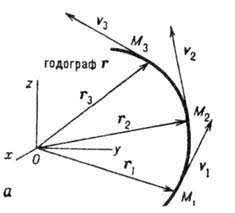
\includegraphics{img/Hodograph.jpg}
		\end{figure}

		$(\lambda_1(t), \lambda_2(t), ..., \lambda_n(t))$ -- координаты точек годографа.
		Отображение $\widetilde{r} : I \to \mathcal{A}$ называется \textit{параметризацией}.

		\item Векторное поле вдоль множества. Пусть дано $\mathcal{A}, \varphi : I \to \mathcal{A}$ -- параметризация, $\overline{r} : I \to \mathbb{V}$ -- вектор-функция.
		
		\begin{figure}[H]
			\centering
			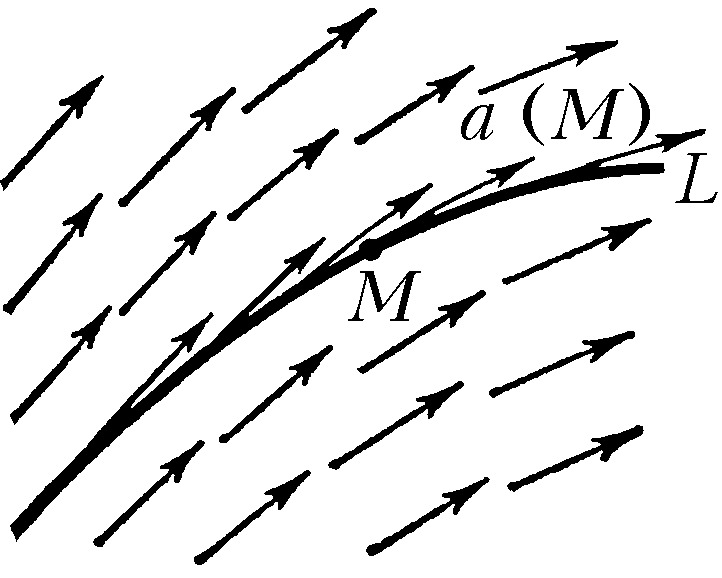
\includegraphics{img/vector_field.jpg}
		\end{figure}
	\end{MyList}
\end{Rem}

\Subsection{Параметризованные гладкие кривые}

\begin{Def}[Гомеоморфизм]
	\textit{Гомеоморфизм} -- биективное непрерывное в обе стороны отображение.
\end{Def}

\begin{Def}[Регулярная гладкая параметризация]
	Пусть $\varphi : I \to \R^n$ -- параметризация кривой. Тогда будем называть её \textit{регулярной гладкой параметризацией}, если
	\begin{MyList}
		\item $\varphi \in C^\infty (I)$ 
		\item $\varphi' \neq 0 \ \forall t$ -- регулярность
		\item $\varphi$ -- гомеоморфизм на образ.  
	\end{MyList}
\end{Def}

\begin{Def}[Элементарная гладкая кривая]
	Множество называется \textit{элементарной гладкой кривой}, если существует её регулярная параметризация.
\end{Def}

\begin{Def}[Гладкая кривая]
	\textit{Гладкая кривая} -- такое множество, что любая точка обладает $\varepsilon$-окрестностью такой, что это множество в этой $\varepsilon$-окрестности является элементарной гладкой кривой.
\end{Def}

\begin{Def}
	Любая точка гладкой кривой обладает $\varepsilon$-окрестностью, в которой она является графиком гладкой функции. 
\end{Def}

\Subsection{Касательные к кривой}

\begin{Thm}
	Пусть $\varphi : I \to \R^n$ -- параметризация, задающая элементарную гладкую кривую, $\varphi(t) = (f_1(t), ..., f_n(t))$.
	Тогда

	\[\varphi'(t) = \lim_{\Delta \to 0} \frac{\varphi(t + \Delta) - \varphi(t)}{\Delta}\]
\end{Thm}

\begin{proof}
	Действительно, поскольку
	\[f_i'(t) = \lim_{\Delta \to 0} \frac{f_i(t + \Delta) - f_i(t)}{\Delta}\]
	то 
	\[\varphi'(t) = \lim_{\Delta \to 0} \left( \frac{f_1(t + \Delta) - f_1(t)}{\Delta}, ..., \frac{f_n(t + \Delta) - f_n(t)}{\Delta}\right)\]
	Тогда по линейности
	\[\varphi'(t) = \lim_{\Delta \to 0} \frac{1}{\Delta} \left(f_1(t + \Delta) - f_1(t), ..., f_n(t + \Delta) - f_n(t)\right) = \lim_{\Delta \to 0} \frac{\varphi(t + \Delta) - \varphi(t)}{\Delta}\]
\end{proof}

\begin{Def}[Касательная к кривой]
	Прямая, содержащая $\varphi'$ называется \textit{касательной}. Касательная является пределом секущих.
\end{Def}

\begin{Def}[Угол между кривыми]
	Угол между пересекающимися гладкими кривыми -- это угол между касательными в точке их пересечения.
\end{Def}

\begin{Rem}
	Угол между кривыми равен
	\[\cos \alpha = \frac{1 + f'(x_0) g'(x_0)}{\sqrt{1 + (f'(x_0)^2)} \cdot \sqrt{1 + (g'(x_0))^2}}\]
\end{Rem}

\begin{Rem}
	Векторное поле на сфере. Задача о Винни-пухе.
\end{Rem}

\Subsection{Длина кривой}

\begin{figure}[H]
	\centering
	\def\svgwidth{.5\columnwidth}
	\input{img/curve_length.pdf_tex}
\end{figure}

\begin{Thm}[Длина дуги]
	Пусть $\varphi : I \to \R^n$. Тогда длина дуги $\varphi(t)$ на $[a, b]$ выражается по формуле
	\[l = \int_{a}^{b} |\varphi'(t)|\,dt\]
\end{Thm}

\begin{proof}
	Разобьем отрезок $[a, b]$ на $N$ равных частей $\varphi(t_i)$, $t_0 = a, t_N = b$.
	Рассмотрим $|\varphi(t_{i + 1}) - \varphi(t_i)|$: это длина хорды кривой, заданной разностью векторов $\varphi(t_{i + 1})$ и $\varphi(t_i)$.
	Рассмотрим длину ломаной, составленной из этих хорд:
	\[S_N = \sum_{i=0}^{N - 1} |\varphi(t_{i + 1}) - \varphi(t_i)|\]
	Если существует $\lim_{N \to \infty} S_N = S$, то $S$ называется \textit{длиной дуги}. Итак, посчитаем предел
	\[\lim_{N \to \infty} S_N = \lim_{N \to \infty} \sum_{i=0}^{N - 1} \left| \frac{\varphi(t_{i + 1}) - \varphi(t_i)}{t_{i + 1} - t_i}\right| \cdot (t_{i + 1} - t_i) = \lim_{\Delta \to 0} \sum\left| \frac{\varphi(t_{i + 1}) - \varphi(t_i)}{\Delta}\right| \Delta\]
	Поверим, что 
	\[\left|\frac{\varphi(t_{i + 1}) - \varphi(t_i)}{\Delta}\right| \cong |\varphi'(\widetilde{t}_i)|\]
	Тогда исходный предел равен
	\[\lim_{\Delta \to 0} \sum |\varphi'(t_i)|\Delta = \int_{t_0}^{t_N} |\varphi'(t)|\,dt\]  
\end{proof}

\begin{Def}
	Дуги, имеющие длину, называются спрямляемыми.
\end{Def}

\end{document}